\documentclass[twoside]{book}

% Packages required by doxygen
\usepackage{fixltx2e}
\usepackage{calc}
\usepackage{doxygen}
\usepackage[export]{adjustbox} % also loads graphicx
\usepackage{graphicx}
\usepackage[utf8]{inputenc}
\usepackage{makeidx}
\usepackage{multicol}
\usepackage{multirow}
\PassOptionsToPackage{warn}{textcomp}
\usepackage{textcomp}
\usepackage[nointegrals]{wasysym}
\usepackage[table]{xcolor}

% Font selection
\usepackage[T1]{fontenc}
\usepackage[scaled=.90]{helvet}
\usepackage{courier}
\usepackage{amssymb}
\usepackage{sectsty}
\renewcommand{\familydefault}{\sfdefault}
\allsectionsfont{%
  \fontseries{bc}\selectfont%
  \color{darkgray}%
}
\renewcommand{\DoxyLabelFont}{%
  \fontseries{bc}\selectfont%
  \color{darkgray}%
}
\newcommand{\+}{\discretionary{\mbox{\scriptsize$\hookleftarrow$}}{}{}}

% Page & text layout
\usepackage{geometry}
\geometry{%
  a4paper,%
  top=2.5cm,%
  bottom=2.5cm,%
  left=2.5cm,%
  right=2.5cm%
}
\tolerance=750
\hfuzz=15pt
\hbadness=750
\setlength{\emergencystretch}{15pt}
\setlength{\parindent}{0cm}
\setlength{\parskip}{3ex plus 2ex minus 2ex}
\makeatletter
\renewcommand{\paragraph}{%
  \@startsection{paragraph}{4}{0ex}{-1.0ex}{1.0ex}{%
    \normalfont\normalsize\bfseries\SS@parafont%
  }%
}
\renewcommand{\subparagraph}{%
  \@startsection{subparagraph}{5}{0ex}{-1.0ex}{1.0ex}{%
    \normalfont\normalsize\bfseries\SS@subparafont%
  }%
}
\makeatother

% Headers & footers
\usepackage{fancyhdr}
\pagestyle{fancyplain}
\fancyhead[LE]{\fancyplain{}{\bfseries\thepage}}
\fancyhead[CE]{\fancyplain{}{}}
\fancyhead[RE]{\fancyplain{}{\bfseries\leftmark}}
\fancyhead[LO]{\fancyplain{}{\bfseries\rightmark}}
\fancyhead[CO]{\fancyplain{}{}}
\fancyhead[RO]{\fancyplain{}{\bfseries\thepage}}
\fancyfoot[LE]{\fancyplain{}{}}
\fancyfoot[CE]{\fancyplain{}{}}
\fancyfoot[RE]{\fancyplain{}{\bfseries\scriptsize Generated by Doxygen }}
\fancyfoot[LO]{\fancyplain{}{\bfseries\scriptsize Generated by Doxygen }}
\fancyfoot[CO]{\fancyplain{}{}}
\fancyfoot[RO]{\fancyplain{}{}}
\renewcommand{\footrulewidth}{0.4pt}
\renewcommand{\chaptermark}[1]{%
  \markboth{#1}{}%
}
\renewcommand{\sectionmark}[1]{%
  \markright{\thesection\ #1}%
}

% Indices & bibliography
\usepackage{natbib}
\usepackage[titles]{tocloft}
\setcounter{tocdepth}{3}
\setcounter{secnumdepth}{5}
\makeindex

% Hyperlinks (required, but should be loaded last)
\usepackage{ifpdf}
\ifpdf
  \usepackage[pdftex,pagebackref=true]{hyperref}
\else
  \usepackage[ps2pdf,pagebackref=true]{hyperref}
\fi
\hypersetup{%
  colorlinks=true,%
  linkcolor=blue,%
  citecolor=blue,%
  unicode%
}

% Custom commands
\newcommand{\clearemptydoublepage}{%
  \newpage{\pagestyle{empty}\cleardoublepage}%
}

\usepackage{caption}
\captionsetup{labelsep=space,justification=centering,font={bf},singlelinecheck=off,skip=4pt,position=top}

%===== C O N T E N T S =====

\begin{document}

% Titlepage & ToC
\hypersetup{pageanchor=false,
             bookmarksnumbered=true,
             pdfencoding=unicode
            }
\pagenumbering{alph}
\begin{titlepage}
\vspace*{7cm}
\begin{center}%
{\Large Practica Animacion 3D \\[1ex]\large 1 }\\
\vspace*{1cm}
{\large Generated by Doxygen 1.8.14}\\
\end{center}
\end{titlepage}
\clearemptydoublepage
\pagenumbering{roman}
\tableofcontents
\clearemptydoublepage
\pagenumbering{arabic}
\hypersetup{pageanchor=true}

%--- Begin generated contents ---
\chapter{Hierarchical Index}
\section{Class Hierarchy}
This inheritance list is sorted roughly, but not completely, alphabetically\+:\begin{DoxyCompactList}
\item \contentsline{section}{Game\+Object}{\pageref{class_game_object}}{}
\begin{DoxyCompactList}
\item \contentsline{section}{Bullet}{\pageref{class_bullet}}{}
\item \contentsline{section}{Floor}{\pageref{class_floor}}{}
\item \contentsline{section}{Key}{\pageref{class_key}}{}
\item \contentsline{section}{Platform\+Move}{\pageref{class_platform_move}}{}
\item \contentsline{section}{Tank}{\pageref{class_tank}}{}
\item \contentsline{section}{Targets}{\pageref{class_targets}}{}
\item \contentsline{section}{Wall}{\pageref{class_wall}}{}
\end{DoxyCompactList}
\item \contentsline{section}{Game\+Object\+:\+:Parts}{\pageref{struct_game_object_1_1_parts}}{}
\item \contentsline{section}{Physics\+World}{\pageref{class_physics_world}}{}
\item \contentsline{section}{Rigidbody}{\pageref{class_rigidbody}}{}
\item \contentsline{section}{Scene}{\pageref{class_scene}}{}
\item \contentsline{section}{Shape}{\pageref{class_shape}}{}
\begin{DoxyCompactList}
\item \contentsline{section}{Box\+Shape}{\pageref{class_box_shape}}{}
\item \contentsline{section}{Cylinder\+Shape}{\pageref{class_cylinder_shape}}{}
\item \contentsline{section}{Sphere\+Shape}{\pageref{class_sphere_shape}}{}
\end{DoxyCompactList}
\end{DoxyCompactList}

\chapter{Class Index}
\section{Class List}
Here are the classes, structs, unions and interfaces with brief descriptions\+:\begin{DoxyCompactList}
\item\contentsline{section}{\mbox{\hyperlink{class_box_shape}{Box\+Shape}} }{\pageref{class_box_shape}}{}
\item\contentsline{section}{\mbox{\hyperlink{class_bullet}{Bullet}} }{\pageref{class_bullet}}{}
\item\contentsline{section}{\mbox{\hyperlink{class_cylinder_shape}{Cylinder\+Shape}} }{\pageref{class_cylinder_shape}}{}
\item\contentsline{section}{\mbox{\hyperlink{class_floor}{Floor}} }{\pageref{class_floor}}{}
\item\contentsline{section}{\mbox{\hyperlink{class_game_object}{Game\+Object}} }{\pageref{class_game_object}}{}
\item\contentsline{section}{\mbox{\hyperlink{class_key}{Key}} }{\pageref{class_key}}{}
\item\contentsline{section}{\mbox{\hyperlink{struct_game_object_1_1_parts}{Game\+Object\+::\+Parts}} }{\pageref{struct_game_object_1_1_parts}}{}
\item\contentsline{section}{\mbox{\hyperlink{class_physics_world}{Physics\+World}} }{\pageref{class_physics_world}}{}
\item\contentsline{section}{\mbox{\hyperlink{class_platform_move}{Platform\+Move}} }{\pageref{class_platform_move}}{}
\item\contentsline{section}{\mbox{\hyperlink{class_rigidbody}{Rigidbody}} }{\pageref{class_rigidbody}}{}
\item\contentsline{section}{\mbox{\hyperlink{class_scene}{Scene}} }{\pageref{class_scene}}{}
\item\contentsline{section}{\mbox{\hyperlink{class_shape}{Shape}} }{\pageref{class_shape}}{}
\item\contentsline{section}{\mbox{\hyperlink{class_sphere_shape}{Sphere\+Shape}} }{\pageref{class_sphere_shape}}{}
\item\contentsline{section}{\mbox{\hyperlink{class_tank}{Tank}} }{\pageref{class_tank}}{}
\item\contentsline{section}{\mbox{\hyperlink{class_targets}{Targets}} }{\pageref{class_targets}}{}
\item\contentsline{section}{\mbox{\hyperlink{class_wall}{Wall}} }{\pageref{class_wall}}{}
\end{DoxyCompactList}

\chapter{File Index}
\section{File List}
Here is a list of all files with brief descriptions\+:\begin{DoxyCompactList}
\item\contentsline{section}{3d/1 rigid bodies/code/\+Headers/\mbox{\hyperlink{_box_shape_8h}{Box\+Shape.\+h}} }{\pageref{_box_shape_8h}}{}
\item\contentsline{section}{3d/1 rigid bodies/code/\+Headers/\mbox{\hyperlink{_box_shape_8hpp}{Box\+Shape.\+hpp}} }{\pageref{_box_shape_8hpp}}{}
\item\contentsline{section}{3d/1 rigid bodies/code/\+Headers/\mbox{\hyperlink{_bullet_8hpp}{Bullet.\+hpp}} }{\pageref{_bullet_8hpp}}{}
\item\contentsline{section}{3d/1 rigid bodies/code/\+Headers/\mbox{\hyperlink{_cylinder_shape_8hpp}{Cylinder\+Shape.\+hpp}} }{\pageref{_cylinder_shape_8hpp}}{}
\item\contentsline{section}{3d/1 rigid bodies/code/\+Headers/\mbox{\hyperlink{_demo_8hpp}{Demo.\+hpp}} }{\pageref{_demo_8hpp}}{}
\item\contentsline{section}{3d/1 rigid bodies/code/\+Headers/\mbox{\hyperlink{_floor_8hpp}{Floor.\+hpp}} }{\pageref{_floor_8hpp}}{}
\item\contentsline{section}{3d/1 rigid bodies/code/\+Headers/\mbox{\hyperlink{_game_object_8hpp}{Game\+Object.\+hpp}} }{\pageref{_game_object_8hpp}}{}
\item\contentsline{section}{3d/1 rigid bodies/code/\+Headers/\mbox{\hyperlink{_key_8hpp}{Key.\+hpp}} }{\pageref{_key_8hpp}}{}
\item\contentsline{section}{3d/1 rigid bodies/code/\+Headers/\mbox{\hyperlink{_physics_world_8hpp}{Physics\+World.\+hpp}} }{\pageref{_physics_world_8hpp}}{}
\item\contentsline{section}{3d/1 rigid bodies/code/\+Headers/\mbox{\hyperlink{_platform_move_8hpp}{Platform\+Move.\+hpp}} }{\pageref{_platform_move_8hpp}}{}
\item\contentsline{section}{3d/1 rigid bodies/code/\+Headers/\mbox{\hyperlink{_rigidbody_8hpp}{Rigidbody.\+hpp}} }{\pageref{_rigidbody_8hpp}}{}
\item\contentsline{section}{3d/1 rigid bodies/code/\+Headers/\mbox{\hyperlink{_scene_8hpp}{Scene.\+hpp}} }{\pageref{_scene_8hpp}}{}
\item\contentsline{section}{3d/1 rigid bodies/code/\+Headers/\mbox{\hyperlink{_shape_8hpp}{Shape.\+hpp}} }{\pageref{_shape_8hpp}}{}
\item\contentsline{section}{3d/1 rigid bodies/code/\+Headers/\mbox{\hyperlink{_sphere_shape_8hpp}{Sphere\+Shape.\+hpp}} }{\pageref{_sphere_shape_8hpp}}{}
\item\contentsline{section}{3d/1 rigid bodies/code/\+Headers/\mbox{\hyperlink{_tank_8hpp}{Tank.\+hpp}} }{\pageref{_tank_8hpp}}{}
\item\contentsline{section}{3d/1 rigid bodies/code/\+Headers/\mbox{\hyperlink{_targets_8hpp}{Targets.\+hpp}} }{\pageref{_targets_8hpp}}{}
\item\contentsline{section}{3d/1 rigid bodies/code/\+Headers/\mbox{\hyperlink{_wall_8hpp}{Wall.\+hpp}} }{\pageref{_wall_8hpp}}{}
\end{DoxyCompactList}

\chapter{Class Documentation}
\hypertarget{class_box_shape}{}\section{Box\+Shape Class Reference}
\label{class_box_shape}\index{Box\+Shape@{Box\+Shape}}


{\ttfamily \#include $<$Box\+Shape.\+hpp$>$}

Inheritance diagram for Box\+Shape\+:\begin{figure}[H]
\begin{center}
\leavevmode
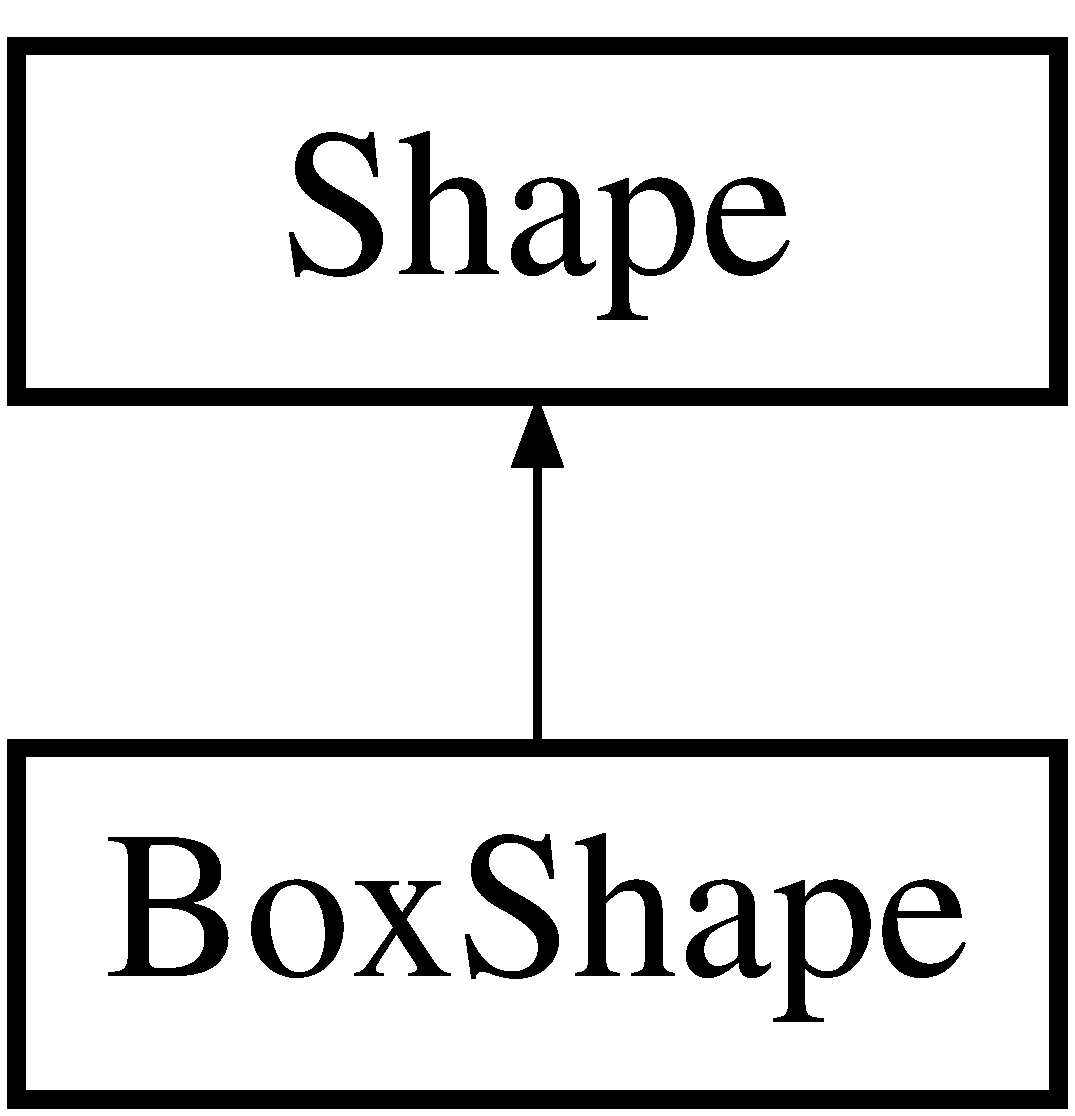
\includegraphics[height=2.000000cm]{class_box_shape}
\end{center}
\end{figure}
\subsection*{Public Member Functions}
\begin{DoxyCompactItemize}
\item 
\mbox{\hyperlink{class_box_shape_a684f14be4d5600b88eb9a10019718097}{Box\+Shape}} (float width, float height, float depth)
\end{DoxyCompactItemize}
\subsection*{Additional Inherited Members}


\subsection{Constructor \& Destructor Documentation}
\mbox{\Hypertarget{class_box_shape_a684f14be4d5600b88eb9a10019718097}\label{class_box_shape_a684f14be4d5600b88eb9a10019718097}} 
\index{Box\+Shape@{Box\+Shape}!Box\+Shape@{Box\+Shape}}
\index{Box\+Shape@{Box\+Shape}!Box\+Shape@{Box\+Shape}}
\subsubsection{\texorpdfstring{Box\+Shape()}{BoxShape()}}
{\footnotesize\ttfamily Box\+Shape\+::\+Box\+Shape (\begin{DoxyParamCaption}\item[{float}]{width,  }\item[{float}]{height,  }\item[{float}]{depth }\end{DoxyParamCaption})\hspace{0.3cm}{\ttfamily [inline]}}



The documentation for this class was generated from the following file\+:\begin{DoxyCompactItemize}
\item 
3d/1 rigid bodies/code/\+Headers/\mbox{\hyperlink{_box_shape_8hpp}{Box\+Shape.\+hpp}}\end{DoxyCompactItemize}

\hypertarget{class_bullet}{}\section{Bullet Class Reference}
\label{class_bullet}\index{Bullet@{Bullet}}


{\ttfamily \#include $<$Bullet.\+hpp$>$}

Inheritance diagram for Bullet\+:\begin{figure}[H]
\begin{center}
\leavevmode
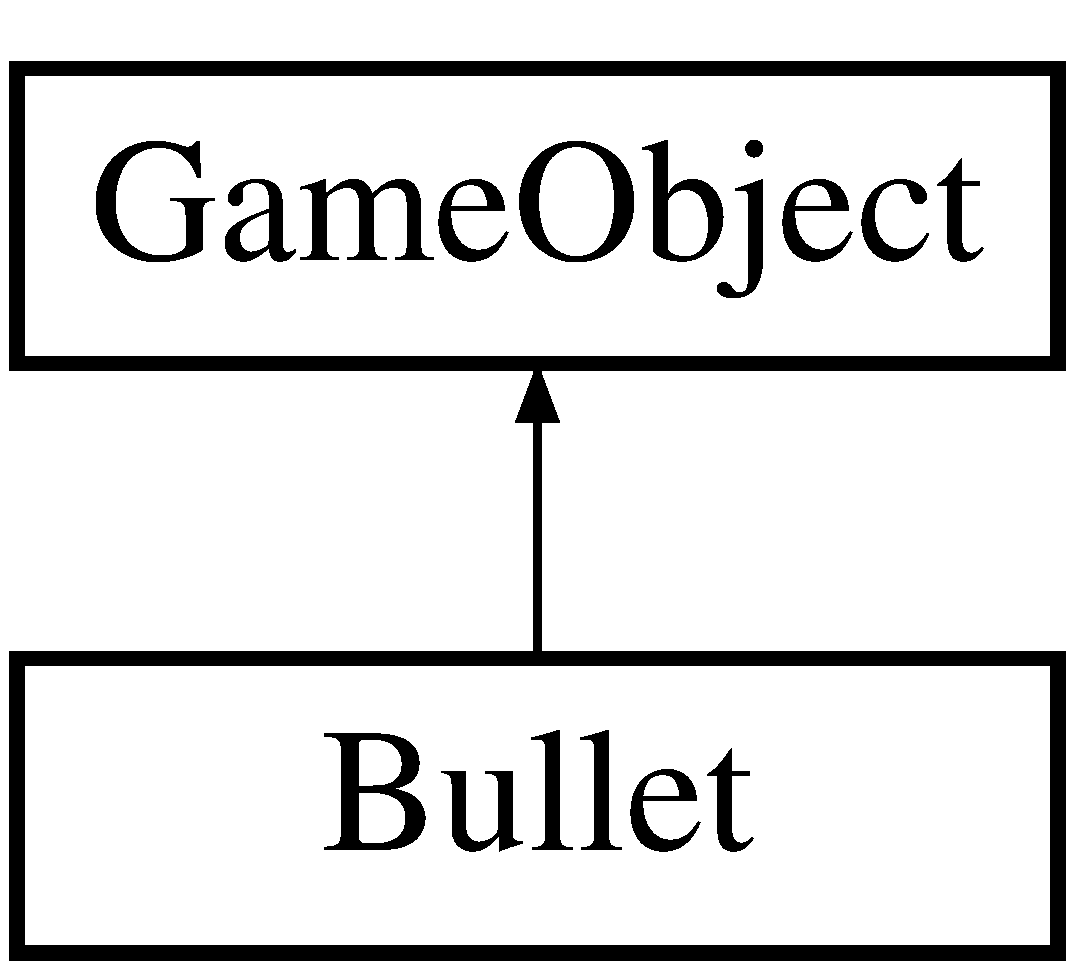
\includegraphics[height=2.000000cm]{class_bullet}
\end{center}
\end{figure}
\subsection*{Public Member Functions}
\begin{DoxyCompactItemize}
\item 
\mbox{\hyperlink{class_bullet_a0e0e8391d068e29f566b4372f03af83a}{Bullet}} (\mbox{\hyperlink{class_scene}{Scene}} \&\mbox{\hyperlink{class_game_object_aeea61de934e13603696b4ed00e9fe42e}{scene}}, int \+\_\+count, bt\+Vector3 \&\+\_\+vector)
\item 
void \mbox{\hyperlink{class_bullet_a4b58c9ddf90ecd78b2e5b292c7496850}{render}} () override
\end{DoxyCompactItemize}
\subsection*{Additional Inherited Members}


\subsection{Constructor \& Destructor Documentation}
\mbox{\Hypertarget{class_bullet_a0e0e8391d068e29f566b4372f03af83a}\label{class_bullet_a0e0e8391d068e29f566b4372f03af83a}} 
\index{Bullet@{Bullet}!Bullet@{Bullet}}
\index{Bullet@{Bullet}!Bullet@{Bullet}}
\subsubsection{\texorpdfstring{Bullet()}{Bullet()}}
{\footnotesize\ttfamily Bullet\+::\+Bullet (\begin{DoxyParamCaption}\item[{\mbox{\hyperlink{class_scene}{Scene}} \&}]{scene,  }\item[{int}]{\+\_\+count,  }\item[{bt\+Vector3 \&}]{\+\_\+vector }\end{DoxyParamCaption})}



\subsection{Member Function Documentation}
\mbox{\Hypertarget{class_bullet_a4b58c9ddf90ecd78b2e5b292c7496850}\label{class_bullet_a4b58c9ddf90ecd78b2e5b292c7496850}} 
\index{Bullet@{Bullet}!render@{render}}
\index{render@{render}!Bullet@{Bullet}}
\subsubsection{\texorpdfstring{render()}{render()}}
{\footnotesize\ttfamily void Bullet\+::render (\begin{DoxyParamCaption}{ }\end{DoxyParamCaption})\hspace{0.3cm}{\ttfamily [override]}, {\ttfamily [virtual]}}



Implements \mbox{\hyperlink{class_game_object_adee58d508cfa907162d1192a25dc21b9}{Game\+Object}}.



The documentation for this class was generated from the following file\+:\begin{DoxyCompactItemize}
\item 
3d/1 rigid bodies/code/\+Headers/\mbox{\hyperlink{_bullet_8hpp}{Bullet.\+hpp}}\end{DoxyCompactItemize}

\hypertarget{class_cylinder_shape}{}\section{Cylinder\+Shape Class Reference}
\label{class_cylinder_shape}\index{Cylinder\+Shape@{Cylinder\+Shape}}


{\ttfamily \#include $<$Cylinder\+Shape.\+hpp$>$}

Inheritance diagram for Cylinder\+Shape\+:\begin{figure}[H]
\begin{center}
\leavevmode
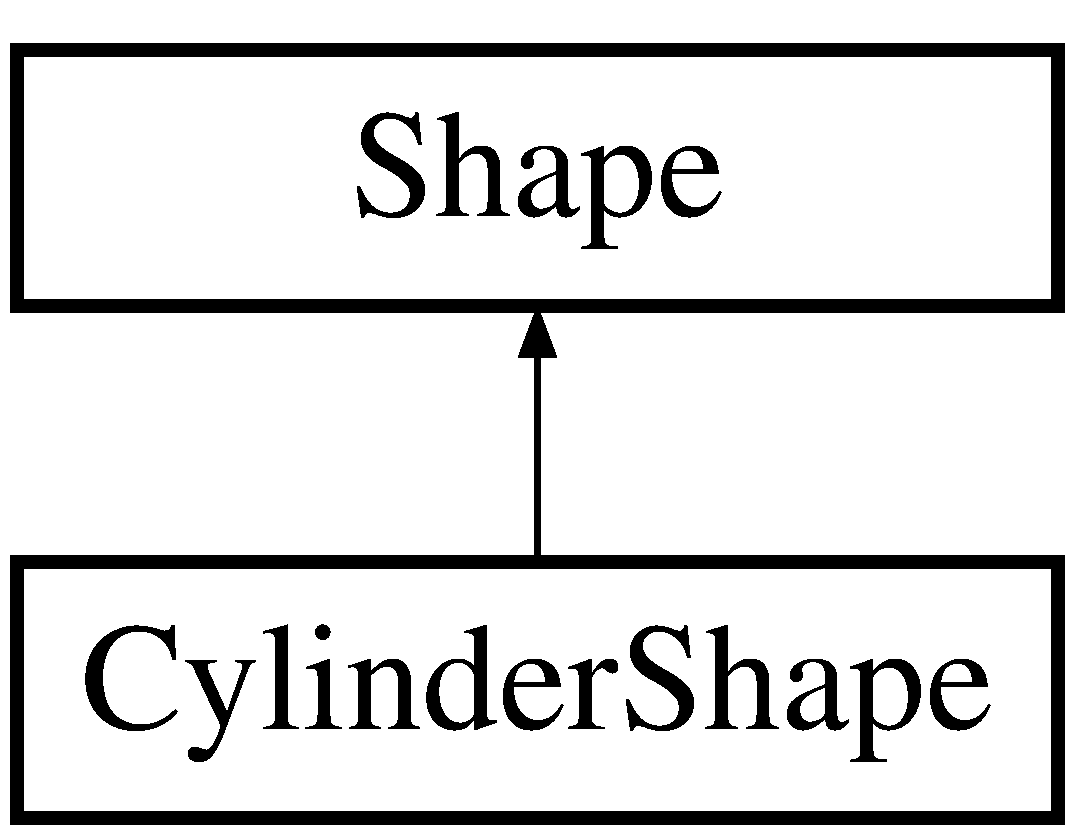
\includegraphics[height=2.000000cm]{class_cylinder_shape}
\end{center}
\end{figure}
\subsection*{Public Member Functions}
\begin{DoxyCompactItemize}
\item 
\mbox{\hyperlink{class_cylinder_shape_a79eaa4cbb70735ffbb23e1890e098dfc}{Cylinder\+Shape}} (float width, float height, float depth)
\end{DoxyCompactItemize}
\subsection*{Additional Inherited Members}


\subsection{Constructor \& Destructor Documentation}
\mbox{\Hypertarget{class_cylinder_shape_a79eaa4cbb70735ffbb23e1890e098dfc}\label{class_cylinder_shape_a79eaa4cbb70735ffbb23e1890e098dfc}} 
\index{Cylinder\+Shape@{Cylinder\+Shape}!Cylinder\+Shape@{Cylinder\+Shape}}
\index{Cylinder\+Shape@{Cylinder\+Shape}!Cylinder\+Shape@{Cylinder\+Shape}}
\subsubsection{\texorpdfstring{Cylinder\+Shape()}{CylinderShape()}}
{\footnotesize\ttfamily Cylinder\+Shape\+::\+Cylinder\+Shape (\begin{DoxyParamCaption}\item[{float}]{width,  }\item[{float}]{height,  }\item[{float}]{depth }\end{DoxyParamCaption})\hspace{0.3cm}{\ttfamily [inline]}}



The documentation for this class was generated from the following file\+:\begin{DoxyCompactItemize}
\item 
3d/1 rigid bodies/code/\+Headers/\mbox{\hyperlink{_cylinder_shape_8hpp}{Cylinder\+Shape.\+hpp}}\end{DoxyCompactItemize}

\hypertarget{class_floor}{}\section{Floor Class Reference}
\label{class_floor}\index{Floor@{Floor}}


{\ttfamily \#include $<$Floor.\+hpp$>$}

Inheritance diagram for Floor\+:\begin{figure}[H]
\begin{center}
\leavevmode
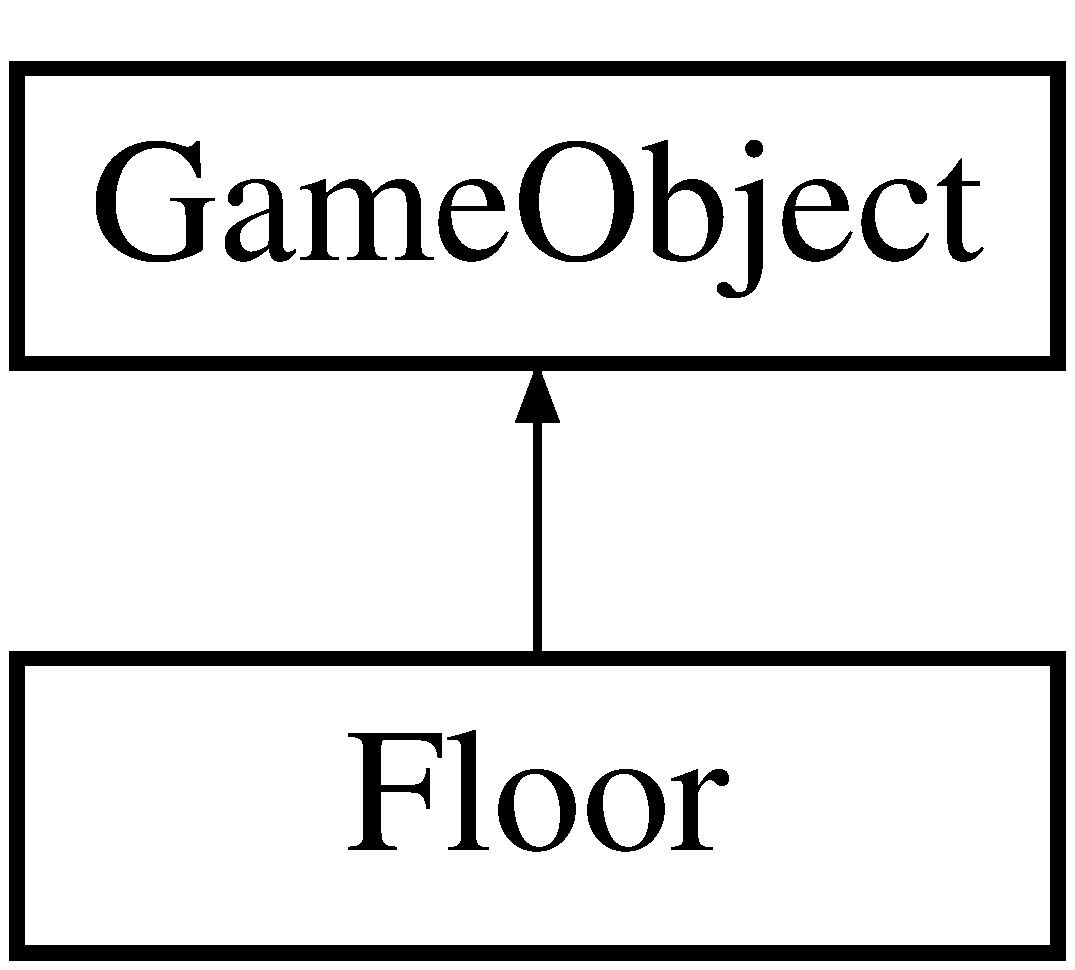
\includegraphics[height=2.000000cm]{class_floor}
\end{center}
\end{figure}
\subsection*{Public Member Functions}
\begin{DoxyCompactItemize}
\item 
\mbox{\hyperlink{class_floor_ac3f66e1dc58f13c12d94200bc1d22caa}{Floor}} (\mbox{\hyperlink{class_scene}{Scene}} \&\mbox{\hyperlink{class_game_object_aeea61de934e13603696b4ed00e9fe42e}{scene}})
\item 
void \mbox{\hyperlink{class_floor_a243d39104b6aacb662481be4fda2d72e}{render}} () override
\end{DoxyCompactItemize}
\subsection*{Additional Inherited Members}


\subsection{Constructor \& Destructor Documentation}
\mbox{\Hypertarget{class_floor_ac3f66e1dc58f13c12d94200bc1d22caa}\label{class_floor_ac3f66e1dc58f13c12d94200bc1d22caa}} 
\index{Floor@{Floor}!Floor@{Floor}}
\index{Floor@{Floor}!Floor@{Floor}}
\subsubsection{\texorpdfstring{Floor()}{Floor()}}
{\footnotesize\ttfamily Floor\+::\+Floor (\begin{DoxyParamCaption}\item[{\mbox{\hyperlink{class_scene}{Scene}} \&}]{scene }\end{DoxyParamCaption})}



\subsection{Member Function Documentation}
\mbox{\Hypertarget{class_floor_a243d39104b6aacb662481be4fda2d72e}\label{class_floor_a243d39104b6aacb662481be4fda2d72e}} 
\index{Floor@{Floor}!render@{render}}
\index{render@{render}!Floor@{Floor}}
\subsubsection{\texorpdfstring{render()}{render()}}
{\footnotesize\ttfamily void Floor\+::render (\begin{DoxyParamCaption}{ }\end{DoxyParamCaption})\hspace{0.3cm}{\ttfamily [override]}, {\ttfamily [virtual]}}



Implements \mbox{\hyperlink{class_game_object_adee58d508cfa907162d1192a25dc21b9}{Game\+Object}}.



The documentation for this class was generated from the following file\+:\begin{DoxyCompactItemize}
\item 
3d/1 rigid bodies/code/\+Headers/\mbox{\hyperlink{_floor_8hpp}{Floor.\+hpp}}\end{DoxyCompactItemize}

\hypertarget{class_game_object}{}\section{Game\+Object Class Reference}
\label{class_game_object}\index{Game\+Object@{Game\+Object}}


{\ttfamily \#include $<$Game\+Object.\+hpp$>$}

Inheritance diagram for Game\+Object\+:\begin{figure}[H]
\begin{center}
\leavevmode
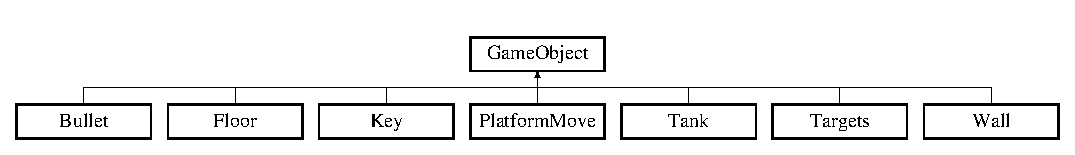
\includegraphics[height=1.632653cm]{class_game_object}
\end{center}
\end{figure}
\subsection*{Classes}
\begin{DoxyCompactItemize}
\item 
struct \mbox{\hyperlink{struct_game_object_1_1_parts}{Parts}}
\end{DoxyCompactItemize}
\subsection*{Public Member Functions}
\begin{DoxyCompactItemize}
\item 
\mbox{\hyperlink{class_game_object_ab2c6683579548906dc8432bbd823fd76}{Game\+Object}} (\mbox{\hyperlink{class_scene}{Scene}} \&\mbox{\hyperlink{class_game_object_aeea61de934e13603696b4ed00e9fe42e}{scene}})
\item 
void \mbox{\hyperlink{class_game_object_a35111561ee0a5dcbd260ae282fbee715}{add\+Model\+And\+Physics}} (const string \&model\+\_\+obj\+\_\+path, shared\+\_\+ptr$<$ \mbox{\hyperlink{class_rigidbody}{Rigidbody}} $>$ \&rigid\+Body, float physics\+To\+Graphics\+Scale, string name\+Part)
\item 
void \mbox{\hyperlink{class_game_object_ac4d09cf168b9ad3e5ba0c31fb7872c76}{add\+Joints}} (string name, shared\+\_\+ptr$<$ \mbox{\hyperlink{class_rigidbody}{Rigidbody}} $>$ \&rgA, shared\+\_\+ptr$<$ \mbox{\hyperlink{class_rigidbody}{Rigidbody}} $>$ \&rgB, bt\+Vector3 \&pivotA, bt\+Vector3 \&pivotB, bt\+Vector3 \&axisA, bt\+Vector3 \&axisB)
\item 
void \mbox{\hyperlink{class_game_object_adad7d284b670db722a2fda8e6a7997e3}{update}} ()
\item 
virtual void \mbox{\hyperlink{class_game_object_adee58d508cfa907162d1192a25dc21b9}{render}} ()=0
\item 
void \mbox{\hyperlink{class_game_object_a514b9b67d7173aba4ed28ddc3e38fd5f}{add\+Parts}} (glt\+::\+Render\+\_\+\+Node \&\+\_\+graphics\+Model, \mbox{\hyperlink{class_physics_world}{Physics\+World}} \&\+\_\+world)
\item 
\mbox{\hyperlink{struct_game_object_1_1_parts}{Parts}} \& \mbox{\hyperlink{class_game_object_a918e94af30ef96eb8a602cf8b0453758}{get\+Parts}} (const std\+::string \&name)
\item 
void \mbox{\hyperlink{class_game_object_a18120b85704277a48ab064138b44e9eb}{add\+Joints\+To\+Physics}} (\mbox{\hyperlink{class_physics_world}{Physics\+World}} \&\+\_\+world)
\item 
\mbox{\hyperlink{class_scene}{Scene}} \& \mbox{\hyperlink{class_game_object_aed20b05219d7b5467dd1978d22fc3361}{get\+Scene}} ()
\item 
bt\+Vector3 \mbox{\hyperlink{class_game_object_a2f7657dbdbe8be16d9ed9c4a4c1c2ef1}{Forward}} (const std\+::string \&name)
\end{DoxyCompactItemize}
\subsection*{Protected Attributes}
\begin{DoxyCompactItemize}
\item 
\mbox{\hyperlink{class_scene}{Scene}} \& \mbox{\hyperlink{class_game_object_aeea61de934e13603696b4ed00e9fe42e}{scene}}
\item 
map$<$ std\+::string, \mbox{\hyperlink{struct_game_object_1_1_parts}{Parts}} $>$ \mbox{\hyperlink{class_game_object_a793b910e9851728a522aba85fe7b829e}{parts}}
\item 
map$<$ string, shared\+\_\+ptr$<$ bt\+Hinge\+Constraint $>$ $>$ \mbox{\hyperlink{class_game_object_ab6ea7ad55d467cc31cd6addf2465f40c}{constrains}}
\end{DoxyCompactItemize}


\subsection{Constructor \& Destructor Documentation}
\mbox{\Hypertarget{class_game_object_ab2c6683579548906dc8432bbd823fd76}\label{class_game_object_ab2c6683579548906dc8432bbd823fd76}} 
\index{Game\+Object@{Game\+Object}!Game\+Object@{Game\+Object}}
\index{Game\+Object@{Game\+Object}!Game\+Object@{Game\+Object}}
\subsubsection{\texorpdfstring{Game\+Object()}{GameObject()}}
{\footnotesize\ttfamily Game\+Object\+::\+Game\+Object (\begin{DoxyParamCaption}\item[{\mbox{\hyperlink{class_scene}{Scene}} \&}]{scene }\end{DoxyParamCaption})\hspace{0.3cm}{\ttfamily [inline]}}



\subsection{Member Function Documentation}
\mbox{\Hypertarget{class_game_object_ac4d09cf168b9ad3e5ba0c31fb7872c76}\label{class_game_object_ac4d09cf168b9ad3e5ba0c31fb7872c76}} 
\index{Game\+Object@{Game\+Object}!add\+Joints@{add\+Joints}}
\index{add\+Joints@{add\+Joints}!Game\+Object@{Game\+Object}}
\subsubsection{\texorpdfstring{add\+Joints()}{addJoints()}}
{\footnotesize\ttfamily void Game\+Object\+::add\+Joints (\begin{DoxyParamCaption}\item[{string}]{name,  }\item[{shared\+\_\+ptr$<$ \mbox{\hyperlink{class_rigidbody}{Rigidbody}} $>$ \&}]{rgA,  }\item[{shared\+\_\+ptr$<$ \mbox{\hyperlink{class_rigidbody}{Rigidbody}} $>$ \&}]{rgB,  }\item[{bt\+Vector3 \&}]{pivotA,  }\item[{bt\+Vector3 \&}]{pivotB,  }\item[{bt\+Vector3 \&}]{axisA,  }\item[{bt\+Vector3 \&}]{axisB }\end{DoxyParamCaption})}

\mbox{\Hypertarget{class_game_object_a18120b85704277a48ab064138b44e9eb}\label{class_game_object_a18120b85704277a48ab064138b44e9eb}} 
\index{Game\+Object@{Game\+Object}!add\+Joints\+To\+Physics@{add\+Joints\+To\+Physics}}
\index{add\+Joints\+To\+Physics@{add\+Joints\+To\+Physics}!Game\+Object@{Game\+Object}}
\subsubsection{\texorpdfstring{add\+Joints\+To\+Physics()}{addJointsToPhysics()}}
{\footnotesize\ttfamily void Game\+Object\+::add\+Joints\+To\+Physics (\begin{DoxyParamCaption}\item[{\mbox{\hyperlink{class_physics_world}{Physics\+World}} \&}]{\+\_\+world }\end{DoxyParamCaption})}

\mbox{\Hypertarget{class_game_object_a35111561ee0a5dcbd260ae282fbee715}\label{class_game_object_a35111561ee0a5dcbd260ae282fbee715}} 
\index{Game\+Object@{Game\+Object}!add\+Model\+And\+Physics@{add\+Model\+And\+Physics}}
\index{add\+Model\+And\+Physics@{add\+Model\+And\+Physics}!Game\+Object@{Game\+Object}}
\subsubsection{\texorpdfstring{add\+Model\+And\+Physics()}{addModelAndPhysics()}}
{\footnotesize\ttfamily void Game\+Object\+::add\+Model\+And\+Physics (\begin{DoxyParamCaption}\item[{const string \&}]{model\+\_\+obj\+\_\+path,  }\item[{shared\+\_\+ptr$<$ \mbox{\hyperlink{class_rigidbody}{Rigidbody}} $>$ \&}]{rigid\+Body,  }\item[{float}]{physics\+To\+Graphics\+Scale,  }\item[{string}]{name\+Part }\end{DoxyParamCaption})}

\mbox{\Hypertarget{class_game_object_a514b9b67d7173aba4ed28ddc3e38fd5f}\label{class_game_object_a514b9b67d7173aba4ed28ddc3e38fd5f}} 
\index{Game\+Object@{Game\+Object}!add\+Parts@{add\+Parts}}
\index{add\+Parts@{add\+Parts}!Game\+Object@{Game\+Object}}
\subsubsection{\texorpdfstring{add\+Parts()}{addParts()}}
{\footnotesize\ttfamily void Game\+Object\+::add\+Parts (\begin{DoxyParamCaption}\item[{glt\+::\+Render\+\_\+\+Node \&}]{\+\_\+graphics\+Model,  }\item[{\mbox{\hyperlink{class_physics_world}{Physics\+World}} \&}]{\+\_\+world }\end{DoxyParamCaption})}

\mbox{\Hypertarget{class_game_object_a2f7657dbdbe8be16d9ed9c4a4c1c2ef1}\label{class_game_object_a2f7657dbdbe8be16d9ed9c4a4c1c2ef1}} 
\index{Game\+Object@{Game\+Object}!Forward@{Forward}}
\index{Forward@{Forward}!Game\+Object@{Game\+Object}}
\subsubsection{\texorpdfstring{Forward()}{Forward()}}
{\footnotesize\ttfamily bt\+Vector3 Game\+Object\+::\+Forward (\begin{DoxyParamCaption}\item[{const std\+::string \&}]{name }\end{DoxyParamCaption})}

\mbox{\Hypertarget{class_game_object_a918e94af30ef96eb8a602cf8b0453758}\label{class_game_object_a918e94af30ef96eb8a602cf8b0453758}} 
\index{Game\+Object@{Game\+Object}!get\+Parts@{get\+Parts}}
\index{get\+Parts@{get\+Parts}!Game\+Object@{Game\+Object}}
\subsubsection{\texorpdfstring{get\+Parts()}{getParts()}}
{\footnotesize\ttfamily \mbox{\hyperlink{struct_game_object_1_1_parts}{Parts}}\& Game\+Object\+::get\+Parts (\begin{DoxyParamCaption}\item[{const std\+::string \&}]{name }\end{DoxyParamCaption})\hspace{0.3cm}{\ttfamily [inline]}}

\mbox{\Hypertarget{class_game_object_aed20b05219d7b5467dd1978d22fc3361}\label{class_game_object_aed20b05219d7b5467dd1978d22fc3361}} 
\index{Game\+Object@{Game\+Object}!get\+Scene@{get\+Scene}}
\index{get\+Scene@{get\+Scene}!Game\+Object@{Game\+Object}}
\subsubsection{\texorpdfstring{get\+Scene()}{getScene()}}
{\footnotesize\ttfamily \mbox{\hyperlink{class_scene}{Scene}}\& Game\+Object\+::get\+Scene (\begin{DoxyParamCaption}{ }\end{DoxyParamCaption})\hspace{0.3cm}{\ttfamily [inline]}}

\mbox{\Hypertarget{class_game_object_adee58d508cfa907162d1192a25dc21b9}\label{class_game_object_adee58d508cfa907162d1192a25dc21b9}} 
\index{Game\+Object@{Game\+Object}!render@{render}}
\index{render@{render}!Game\+Object@{Game\+Object}}
\subsubsection{\texorpdfstring{render()}{render()}}
{\footnotesize\ttfamily virtual void Game\+Object\+::render (\begin{DoxyParamCaption}{ }\end{DoxyParamCaption})\hspace{0.3cm}{\ttfamily [pure virtual]}}



Implemented in \mbox{\hyperlink{class_tank_a9628f999ddc963311cebf069da363d5c}{Tank}}, \mbox{\hyperlink{class_bullet_a4b58c9ddf90ecd78b2e5b292c7496850}{Bullet}}, \mbox{\hyperlink{class_key_ad7047dce6eba1702bf776cb6ffeab3a6}{Key}}, \mbox{\hyperlink{class_platform_move_ac8e703c3529c602c9f0cc0a4148bcc34}{Platform\+Move}}, \mbox{\hyperlink{class_targets_ae4f6dccb119a885728dc9e9c3e287c95}{Targets}}, \mbox{\hyperlink{class_wall_ad2b19eb994789ac7588b61a7ad0d928f}{Wall}}, and \mbox{\hyperlink{class_floor_a243d39104b6aacb662481be4fda2d72e}{Floor}}.

\mbox{\Hypertarget{class_game_object_adad7d284b670db722a2fda8e6a7997e3}\label{class_game_object_adad7d284b670db722a2fda8e6a7997e3}} 
\index{Game\+Object@{Game\+Object}!update@{update}}
\index{update@{update}!Game\+Object@{Game\+Object}}
\subsubsection{\texorpdfstring{update()}{update()}}
{\footnotesize\ttfamily void Game\+Object\+::update (\begin{DoxyParamCaption}{ }\end{DoxyParamCaption})}



\subsection{Member Data Documentation}
\mbox{\Hypertarget{class_game_object_ab6ea7ad55d467cc31cd6addf2465f40c}\label{class_game_object_ab6ea7ad55d467cc31cd6addf2465f40c}} 
\index{Game\+Object@{Game\+Object}!constrains@{constrains}}
\index{constrains@{constrains}!Game\+Object@{Game\+Object}}
\subsubsection{\texorpdfstring{constrains}{constrains}}
{\footnotesize\ttfamily map$<$ string, shared\+\_\+ptr$<$bt\+Hinge\+Constraint$>$ $>$ Game\+Object\+::constrains\hspace{0.3cm}{\ttfamily [protected]}}

\mbox{\Hypertarget{class_game_object_a793b910e9851728a522aba85fe7b829e}\label{class_game_object_a793b910e9851728a522aba85fe7b829e}} 
\index{Game\+Object@{Game\+Object}!parts@{parts}}
\index{parts@{parts}!Game\+Object@{Game\+Object}}
\subsubsection{\texorpdfstring{parts}{parts}}
{\footnotesize\ttfamily map$<$ std\+::string, \mbox{\hyperlink{struct_game_object_1_1_parts}{Parts}} $>$ Game\+Object\+::parts\hspace{0.3cm}{\ttfamily [protected]}}

\mbox{\Hypertarget{class_game_object_aeea61de934e13603696b4ed00e9fe42e}\label{class_game_object_aeea61de934e13603696b4ed00e9fe42e}} 
\index{Game\+Object@{Game\+Object}!scene@{scene}}
\index{scene@{scene}!Game\+Object@{Game\+Object}}
\subsubsection{\texorpdfstring{scene}{scene}}
{\footnotesize\ttfamily \mbox{\hyperlink{class_scene}{Scene}}\& Game\+Object\+::scene\hspace{0.3cm}{\ttfamily [protected]}}



The documentation for this class was generated from the following file\+:\begin{DoxyCompactItemize}
\item 
3d/1 rigid bodies/code/\+Headers/\mbox{\hyperlink{_game_object_8hpp}{Game\+Object.\+hpp}}\end{DoxyCompactItemize}

\hypertarget{class_key}{}\section{Key Class Reference}
\label{class_key}\index{Key@{Key}}


{\ttfamily \#include $<$Key.\+hpp$>$}

Inheritance diagram for Key\+:\begin{figure}[H]
\begin{center}
\leavevmode
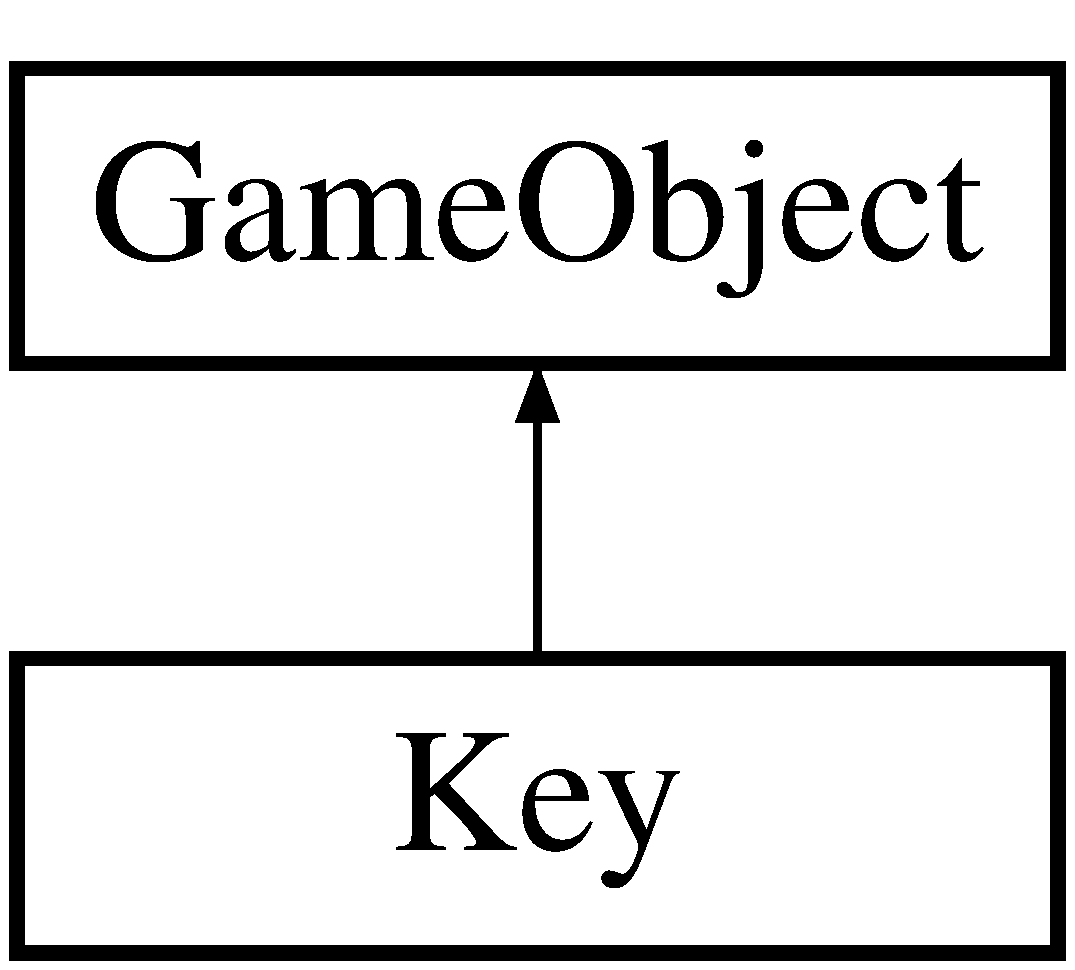
\includegraphics[height=2.000000cm]{class_key}
\end{center}
\end{figure}
\subsection*{Public Member Functions}
\begin{DoxyCompactItemize}
\item 
\mbox{\hyperlink{class_key_aaf6863a25f5bff8c2e090d2742bdd8c7}{Key}} (\mbox{\hyperlink{class_scene}{Scene}} \&\mbox{\hyperlink{class_game_object_aeea61de934e13603696b4ed00e9fe42e}{scene}})
\item 
void \mbox{\hyperlink{class_key_ad7047dce6eba1702bf776cb6ffeab3a6}{render}} () override
\item 
void \mbox{\hyperlink{class_key_a6c31c0a20e5bcb5a3e0399498b9d0c14}{delete\+Key}} ()
\end{DoxyCompactItemize}
\subsection*{Additional Inherited Members}


\subsection{Constructor \& Destructor Documentation}
\mbox{\Hypertarget{class_key_aaf6863a25f5bff8c2e090d2742bdd8c7}\label{class_key_aaf6863a25f5bff8c2e090d2742bdd8c7}} 
\index{Key@{Key}!Key@{Key}}
\index{Key@{Key}!Key@{Key}}
\subsubsection{\texorpdfstring{Key()}{Key()}}
{\footnotesize\ttfamily Key\+::\+Key (\begin{DoxyParamCaption}\item[{\mbox{\hyperlink{class_scene}{Scene}} \&}]{scene }\end{DoxyParamCaption})}



\subsection{Member Function Documentation}
\mbox{\Hypertarget{class_key_a6c31c0a20e5bcb5a3e0399498b9d0c14}\label{class_key_a6c31c0a20e5bcb5a3e0399498b9d0c14}} 
\index{Key@{Key}!delete\+Key@{delete\+Key}}
\index{delete\+Key@{delete\+Key}!Key@{Key}}
\subsubsection{\texorpdfstring{delete\+Key()}{deleteKey()}}
{\footnotesize\ttfamily void Key\+::delete\+Key (\begin{DoxyParamCaption}{ }\end{DoxyParamCaption})}

\mbox{\Hypertarget{class_key_ad7047dce6eba1702bf776cb6ffeab3a6}\label{class_key_ad7047dce6eba1702bf776cb6ffeab3a6}} 
\index{Key@{Key}!render@{render}}
\index{render@{render}!Key@{Key}}
\subsubsection{\texorpdfstring{render()}{render()}}
{\footnotesize\ttfamily void Key\+::render (\begin{DoxyParamCaption}{ }\end{DoxyParamCaption})\hspace{0.3cm}{\ttfamily [override]}, {\ttfamily [virtual]}}



Implements \mbox{\hyperlink{class_game_object_adee58d508cfa907162d1192a25dc21b9}{Game\+Object}}.



The documentation for this class was generated from the following file\+:\begin{DoxyCompactItemize}
\item 
3d/1 rigid bodies/code/\+Headers/\mbox{\hyperlink{_key_8hpp}{Key.\+hpp}}\end{DoxyCompactItemize}

\hypertarget{struct_game_object_1_1_parts}{}\section{Game\+Object\+:\+:Parts Struct Reference}
\label{struct_game_object_1_1_parts}\index{Game\+Object\+::\+Parts@{Game\+Object\+::\+Parts}}


{\ttfamily \#include $<$Game\+Object.\+hpp$>$}

\subsection*{Public Attributes}
\begin{DoxyCompactItemize}
\item 
shared\+\_\+ptr$<$ \mbox{\hyperlink{class_rigidbody}{Rigidbody}} $>$ \mbox{\hyperlink{struct_game_object_1_1_parts_ac118274639b83227dbce5cd23008660a}{physics\+Body}}
\item 
shared\+\_\+ptr$<$ Model\+\_\+\+Obj $>$ \mbox{\hyperlink{struct_game_object_1_1_parts_a620574a4a1e9cec0d1a11dc70206e636}{graphics\+Model}}
\item 
float \mbox{\hyperlink{struct_game_object_1_1_parts_a898129420b23efe2ed98f1e63a21c1e9}{physics\+To\+Graphics\+Scale}}
\end{DoxyCompactItemize}


\subsection{Member Data Documentation}
\mbox{\Hypertarget{struct_game_object_1_1_parts_a620574a4a1e9cec0d1a11dc70206e636}\label{struct_game_object_1_1_parts_a620574a4a1e9cec0d1a11dc70206e636}} 
\index{Game\+Object\+::\+Parts@{Game\+Object\+::\+Parts}!graphics\+Model@{graphics\+Model}}
\index{graphics\+Model@{graphics\+Model}!Game\+Object\+::\+Parts@{Game\+Object\+::\+Parts}}
\subsubsection{\texorpdfstring{graphics\+Model}{graphicsModel}}
{\footnotesize\ttfamily shared\+\_\+ptr$<$ Model\+\_\+\+Obj $>$ Game\+Object\+::\+Parts\+::graphics\+Model}

\mbox{\Hypertarget{struct_game_object_1_1_parts_ac118274639b83227dbce5cd23008660a}\label{struct_game_object_1_1_parts_ac118274639b83227dbce5cd23008660a}} 
\index{Game\+Object\+::\+Parts@{Game\+Object\+::\+Parts}!physics\+Body@{physics\+Body}}
\index{physics\+Body@{physics\+Body}!Game\+Object\+::\+Parts@{Game\+Object\+::\+Parts}}
\subsubsection{\texorpdfstring{physics\+Body}{physicsBody}}
{\footnotesize\ttfamily shared\+\_\+ptr$<$ \mbox{\hyperlink{class_rigidbody}{Rigidbody}} $>$ Game\+Object\+::\+Parts\+::physics\+Body}

\mbox{\Hypertarget{struct_game_object_1_1_parts_a898129420b23efe2ed98f1e63a21c1e9}\label{struct_game_object_1_1_parts_a898129420b23efe2ed98f1e63a21c1e9}} 
\index{Game\+Object\+::\+Parts@{Game\+Object\+::\+Parts}!physics\+To\+Graphics\+Scale@{physics\+To\+Graphics\+Scale}}
\index{physics\+To\+Graphics\+Scale@{physics\+To\+Graphics\+Scale}!Game\+Object\+::\+Parts@{Game\+Object\+::\+Parts}}
\subsubsection{\texorpdfstring{physics\+To\+Graphics\+Scale}{physicsToGraphicsScale}}
{\footnotesize\ttfamily float Game\+Object\+::\+Parts\+::physics\+To\+Graphics\+Scale}



The documentation for this struct was generated from the following file\+:\begin{DoxyCompactItemize}
\item 
3d/1 rigid bodies/code/\+Headers/\mbox{\hyperlink{_game_object_8hpp}{Game\+Object.\+hpp}}\end{DoxyCompactItemize}

\hypertarget{class_physics_world}{}\section{Physics\+World Class Reference}
\label{class_physics_world}\index{Physics\+World@{Physics\+World}}


{\ttfamily \#include $<$Physics\+World.\+hpp$>$}

\subsection*{Public Member Functions}
\begin{DoxyCompactItemize}
\item 
\mbox{\hyperlink{class_physics_world_ae7aea476bf3c5d337a4fa5c1ff02f5d4}{Physics\+World}} ()
\item 
\mbox{\hyperlink{class_physics_world_abf1573b008b52b60a83a8f36cbdd51bc}{$\sim$\+Physics\+World}} ()
\item 
bt\+Discrete\+Dynamics\+World $\ast$ \mbox{\hyperlink{class_physics_world_a494deb5de66fb39a88ebccf48fc9c169}{get\+World}} ()
\item 
void \mbox{\hyperlink{class_physics_world_a37e286968a0f32f62d8a387253490a02}{step}} (float time)
\item 
void \mbox{\hyperlink{class_physics_world_aeef0fd2046bc496955484ec95570eb55}{add\+Rigid\+Body}} (std\+::shared\+\_\+ptr$<$ \mbox{\hyperlink{class_rigidbody}{Rigidbody}} $>$ \&rigid\+Body)
\item 
void \mbox{\hyperlink{class_physics_world_a99a91339a05c64b602031fe899245777}{reset\+World}} ()
\item 
void \mbox{\hyperlink{class_physics_world_a87bdd79dbd912e814980a9ef2108bfad}{add\+Constraint}} (std\+::shared\+\_\+ptr$<$ bt\+Hinge\+Constraint $>$ \+\_\+contraint)
\end{DoxyCompactItemize}


\subsection{Constructor \& Destructor Documentation}
\mbox{\Hypertarget{class_physics_world_ae7aea476bf3c5d337a4fa5c1ff02f5d4}\label{class_physics_world_ae7aea476bf3c5d337a4fa5c1ff02f5d4}} 
\index{Physics\+World@{Physics\+World}!Physics\+World@{Physics\+World}}
\index{Physics\+World@{Physics\+World}!Physics\+World@{Physics\+World}}
\subsubsection{\texorpdfstring{Physics\+World()}{PhysicsWorld()}}
{\footnotesize\ttfamily Physics\+World\+::\+Physics\+World (\begin{DoxyParamCaption}{ }\end{DoxyParamCaption})}

\mbox{\Hypertarget{class_physics_world_abf1573b008b52b60a83a8f36cbdd51bc}\label{class_physics_world_abf1573b008b52b60a83a8f36cbdd51bc}} 
\index{Physics\+World@{Physics\+World}!````~Physics\+World@{$\sim$\+Physics\+World}}
\index{````~Physics\+World@{$\sim$\+Physics\+World}!Physics\+World@{Physics\+World}}
\subsubsection{\texorpdfstring{$\sim$\+Physics\+World()}{~PhysicsWorld()}}
{\footnotesize\ttfamily Physics\+World\+::$\sim$\+Physics\+World (\begin{DoxyParamCaption}{ }\end{DoxyParamCaption})}



\subsection{Member Function Documentation}
\mbox{\Hypertarget{class_physics_world_a87bdd79dbd912e814980a9ef2108bfad}\label{class_physics_world_a87bdd79dbd912e814980a9ef2108bfad}} 
\index{Physics\+World@{Physics\+World}!add\+Constraint@{add\+Constraint}}
\index{add\+Constraint@{add\+Constraint}!Physics\+World@{Physics\+World}}
\subsubsection{\texorpdfstring{add\+Constraint()}{addConstraint()}}
{\footnotesize\ttfamily void Physics\+World\+::add\+Constraint (\begin{DoxyParamCaption}\item[{std\+::shared\+\_\+ptr$<$ bt\+Hinge\+Constraint $>$}]{\+\_\+contraint }\end{DoxyParamCaption})\hspace{0.3cm}{\ttfamily [inline]}}

\mbox{\Hypertarget{class_physics_world_aeef0fd2046bc496955484ec95570eb55}\label{class_physics_world_aeef0fd2046bc496955484ec95570eb55}} 
\index{Physics\+World@{Physics\+World}!add\+Rigid\+Body@{add\+Rigid\+Body}}
\index{add\+Rigid\+Body@{add\+Rigid\+Body}!Physics\+World@{Physics\+World}}
\subsubsection{\texorpdfstring{add\+Rigid\+Body()}{addRigidBody()}}
{\footnotesize\ttfamily void Physics\+World\+::add\+Rigid\+Body (\begin{DoxyParamCaption}\item[{std\+::shared\+\_\+ptr$<$ \mbox{\hyperlink{class_rigidbody}{Rigidbody}} $>$ \&}]{rigid\+Body }\end{DoxyParamCaption})\hspace{0.3cm}{\ttfamily [inline]}}

\mbox{\Hypertarget{class_physics_world_a494deb5de66fb39a88ebccf48fc9c169}\label{class_physics_world_a494deb5de66fb39a88ebccf48fc9c169}} 
\index{Physics\+World@{Physics\+World}!get\+World@{get\+World}}
\index{get\+World@{get\+World}!Physics\+World@{Physics\+World}}
\subsubsection{\texorpdfstring{get\+World()}{getWorld()}}
{\footnotesize\ttfamily bt\+Discrete\+Dynamics\+World$\ast$ Physics\+World\+::get\+World (\begin{DoxyParamCaption}{ }\end{DoxyParamCaption})\hspace{0.3cm}{\ttfamily [inline]}}

\mbox{\Hypertarget{class_physics_world_a99a91339a05c64b602031fe899245777}\label{class_physics_world_a99a91339a05c64b602031fe899245777}} 
\index{Physics\+World@{Physics\+World}!reset\+World@{reset\+World}}
\index{reset\+World@{reset\+World}!Physics\+World@{Physics\+World}}
\subsubsection{\texorpdfstring{reset\+World()}{resetWorld()}}
{\footnotesize\ttfamily void Physics\+World\+::reset\+World (\begin{DoxyParamCaption}{ }\end{DoxyParamCaption})\hspace{0.3cm}{\ttfamily [inline]}}

\mbox{\Hypertarget{class_physics_world_a37e286968a0f32f62d8a387253490a02}\label{class_physics_world_a37e286968a0f32f62d8a387253490a02}} 
\index{Physics\+World@{Physics\+World}!step@{step}}
\index{step@{step}!Physics\+World@{Physics\+World}}
\subsubsection{\texorpdfstring{step()}{step()}}
{\footnotesize\ttfamily void Physics\+World\+::step (\begin{DoxyParamCaption}\item[{float}]{time }\end{DoxyParamCaption})\hspace{0.3cm}{\ttfamily [inline]}}



The documentation for this class was generated from the following file\+:\begin{DoxyCompactItemize}
\item 
3d/1 rigid bodies/code/\+Headers/\mbox{\hyperlink{_physics_world_8hpp}{Physics\+World.\+hpp}}\end{DoxyCompactItemize}

\hypertarget{class_platform_move}{}\section{Platform\+Move Class Reference}
\label{class_platform_move}\index{Platform\+Move@{Platform\+Move}}


{\ttfamily \#include $<$Platform\+Move.\+hpp$>$}

Inheritance diagram for Platform\+Move\+:\begin{figure}[H]
\begin{center}
\leavevmode
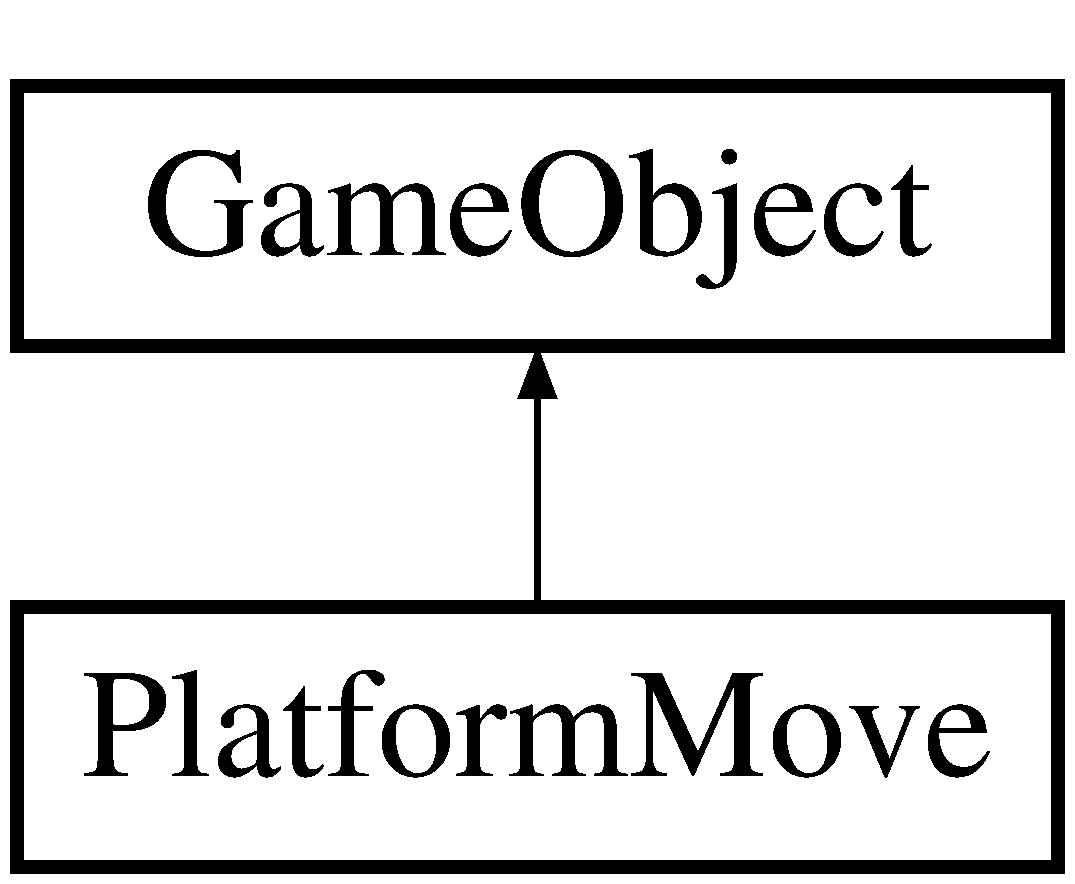
\includegraphics[height=2.000000cm]{class_platform_move}
\end{center}
\end{figure}
\subsection*{Public Member Functions}
\begin{DoxyCompactItemize}
\item 
\mbox{\hyperlink{class_platform_move_a508de74ec711e79d4ce42219eb7d563a}{Platform\+Move}} (\mbox{\hyperlink{class_scene}{Scene}} \&\mbox{\hyperlink{class_game_object_aeea61de934e13603696b4ed00e9fe42e}{scene}})
\item 
void \mbox{\hyperlink{class_platform_move_ac8e703c3529c602c9f0cc0a4148bcc34}{render}} () override
\end{DoxyCompactItemize}
\subsection*{Additional Inherited Members}


\subsection{Constructor \& Destructor Documentation}
\mbox{\Hypertarget{class_platform_move_a508de74ec711e79d4ce42219eb7d563a}\label{class_platform_move_a508de74ec711e79d4ce42219eb7d563a}} 
\index{Platform\+Move@{Platform\+Move}!Platform\+Move@{Platform\+Move}}
\index{Platform\+Move@{Platform\+Move}!Platform\+Move@{Platform\+Move}}
\subsubsection{\texorpdfstring{Platform\+Move()}{PlatformMove()}}
{\footnotesize\ttfamily Platform\+Move\+::\+Platform\+Move (\begin{DoxyParamCaption}\item[{\mbox{\hyperlink{class_scene}{Scene}} \&}]{scene }\end{DoxyParamCaption})}



\subsection{Member Function Documentation}
\mbox{\Hypertarget{class_platform_move_ac8e703c3529c602c9f0cc0a4148bcc34}\label{class_platform_move_ac8e703c3529c602c9f0cc0a4148bcc34}} 
\index{Platform\+Move@{Platform\+Move}!render@{render}}
\index{render@{render}!Platform\+Move@{Platform\+Move}}
\subsubsection{\texorpdfstring{render()}{render()}}
{\footnotesize\ttfamily void Platform\+Move\+::render (\begin{DoxyParamCaption}{ }\end{DoxyParamCaption})\hspace{0.3cm}{\ttfamily [override]}, {\ttfamily [virtual]}}



Implements \mbox{\hyperlink{class_game_object_adee58d508cfa907162d1192a25dc21b9}{Game\+Object}}.



The documentation for this class was generated from the following file\+:\begin{DoxyCompactItemize}
\item 
3d/1 rigid bodies/code/\+Headers/\mbox{\hyperlink{_platform_move_8hpp}{Platform\+Move.\+hpp}}\end{DoxyCompactItemize}

\hypertarget{class_rigidbody}{}\section{Rigidbody Class Reference}
\label{class_rigidbody}\index{Rigidbody@{Rigidbody}}


{\ttfamily \#include $<$Rigidbody.\+hpp$>$}

\subsection*{Public Member Functions}
\begin{DoxyCompactItemize}
\item 
\mbox{\hyperlink{class_rigidbody_a583313febf979a0e72cbc59a5fcc2ab4}{Rigidbody}} (shared\+\_\+ptr$<$ \mbox{\hyperlink{class_shape}{Shape}} $>$ \&\mbox{\hyperlink{class_rigidbody_a817fb8d0991858bd31bdaf8f60df1346}{shape}}, float X, float Y, float Z, bool is\+Static, float mass, float rotateX, float rotateY, float rotateZ)
\item 
virtual \mbox{\hyperlink{class_rigidbody_aeacb70ba57d80c85cfb6f5f50ebecf96}{$\sim$\+Rigidbody}} ()=default
\item 
bt\+Rigid\+Body $\ast$ \mbox{\hyperlink{class_rigidbody_a189022541bfdf0717639e681934f996d}{get}} ()
\item 
bt\+Transform \mbox{\hyperlink{class_rigidbody_a4e63ac1ae27de4b0c84e6a3956fc0edd}{get\+Transform}} ()
\end{DoxyCompactItemize}
\subsection*{Protected Attributes}
\begin{DoxyCompactItemize}
\item 
shared\+\_\+ptr$<$ bt\+Rigid\+Body $>$ \mbox{\hyperlink{class_rigidbody_adc3e81959384b3b97c786805592a36c3}{body}}
\item 
shared\+\_\+ptr$<$ bt\+Default\+Motion\+State $>$ \mbox{\hyperlink{class_rigidbody_a532632942cea50d9f5eb89da3f017777}{state}}
\item 
shared\+\_\+ptr$<$ \mbox{\hyperlink{class_shape}{Shape}} $>$ \mbox{\hyperlink{class_rigidbody_a817fb8d0991858bd31bdaf8f60df1346}{shape}}
\item 
float \mbox{\hyperlink{class_rigidbody_abe7f1cec1c81ff1c0544cdb49ca8cded}{coordX}}
\item 
float \mbox{\hyperlink{class_rigidbody_a6bb882de91a461cc33c7212f53ec0289}{coordY}}
\item 
float \mbox{\hyperlink{class_rigidbody_a7bac1a0470551f7fec7884b68742a8f3}{coordZ}}
\item 
bt\+Transform \mbox{\hyperlink{class_rigidbody_acb3059a56e65ec7e6a8e59462c6023e4}{transform}}
\end{DoxyCompactItemize}


\subsection{Constructor \& Destructor Documentation}
\mbox{\Hypertarget{class_rigidbody_a583313febf979a0e72cbc59a5fcc2ab4}\label{class_rigidbody_a583313febf979a0e72cbc59a5fcc2ab4}} 
\index{Rigidbody@{Rigidbody}!Rigidbody@{Rigidbody}}
\index{Rigidbody@{Rigidbody}!Rigidbody@{Rigidbody}}
\subsubsection{\texorpdfstring{Rigidbody()}{Rigidbody()}}
{\footnotesize\ttfamily Rigidbody\+::\+Rigidbody (\begin{DoxyParamCaption}\item[{shared\+\_\+ptr$<$ \mbox{\hyperlink{class_shape}{Shape}} $>$ \&}]{shape,  }\item[{float}]{X,  }\item[{float}]{Y,  }\item[{float}]{Z,  }\item[{bool}]{is\+Static,  }\item[{float}]{mass,  }\item[{float}]{rotateX,  }\item[{float}]{rotateY,  }\item[{float}]{rotateZ }\end{DoxyParamCaption})}

\mbox{\Hypertarget{class_rigidbody_aeacb70ba57d80c85cfb6f5f50ebecf96}\label{class_rigidbody_aeacb70ba57d80c85cfb6f5f50ebecf96}} 
\index{Rigidbody@{Rigidbody}!````~Rigidbody@{$\sim$\+Rigidbody}}
\index{````~Rigidbody@{$\sim$\+Rigidbody}!Rigidbody@{Rigidbody}}
\subsubsection{\texorpdfstring{$\sim$\+Rigidbody()}{~Rigidbody()}}
{\footnotesize\ttfamily virtual Rigidbody\+::$\sim$\+Rigidbody (\begin{DoxyParamCaption}{ }\end{DoxyParamCaption})\hspace{0.3cm}{\ttfamily [virtual]}, {\ttfamily [default]}}



\subsection{Member Function Documentation}
\mbox{\Hypertarget{class_rigidbody_a189022541bfdf0717639e681934f996d}\label{class_rigidbody_a189022541bfdf0717639e681934f996d}} 
\index{Rigidbody@{Rigidbody}!get@{get}}
\index{get@{get}!Rigidbody@{Rigidbody}}
\subsubsection{\texorpdfstring{get()}{get()}}
{\footnotesize\ttfamily bt\+Rigid\+Body$\ast$ Rigidbody\+::get (\begin{DoxyParamCaption}{ }\end{DoxyParamCaption})\hspace{0.3cm}{\ttfamily [inline]}}

\mbox{\Hypertarget{class_rigidbody_a4e63ac1ae27de4b0c84e6a3956fc0edd}\label{class_rigidbody_a4e63ac1ae27de4b0c84e6a3956fc0edd}} 
\index{Rigidbody@{Rigidbody}!get\+Transform@{get\+Transform}}
\index{get\+Transform@{get\+Transform}!Rigidbody@{Rigidbody}}
\subsubsection{\texorpdfstring{get\+Transform()}{getTransform()}}
{\footnotesize\ttfamily bt\+Transform Rigidbody\+::get\+Transform (\begin{DoxyParamCaption}{ }\end{DoxyParamCaption})\hspace{0.3cm}{\ttfamily [inline]}}



\subsection{Member Data Documentation}
\mbox{\Hypertarget{class_rigidbody_adc3e81959384b3b97c786805592a36c3}\label{class_rigidbody_adc3e81959384b3b97c786805592a36c3}} 
\index{Rigidbody@{Rigidbody}!body@{body}}
\index{body@{body}!Rigidbody@{Rigidbody}}
\subsubsection{\texorpdfstring{body}{body}}
{\footnotesize\ttfamily shared\+\_\+ptr$<$ bt\+Rigid\+Body $>$ Rigidbody\+::body\hspace{0.3cm}{\ttfamily [protected]}}

\mbox{\Hypertarget{class_rigidbody_abe7f1cec1c81ff1c0544cdb49ca8cded}\label{class_rigidbody_abe7f1cec1c81ff1c0544cdb49ca8cded}} 
\index{Rigidbody@{Rigidbody}!coordX@{coordX}}
\index{coordX@{coordX}!Rigidbody@{Rigidbody}}
\subsubsection{\texorpdfstring{coordX}{coordX}}
{\footnotesize\ttfamily float Rigidbody\+::coordX\hspace{0.3cm}{\ttfamily [protected]}}

\mbox{\Hypertarget{class_rigidbody_a6bb882de91a461cc33c7212f53ec0289}\label{class_rigidbody_a6bb882de91a461cc33c7212f53ec0289}} 
\index{Rigidbody@{Rigidbody}!coordY@{coordY}}
\index{coordY@{coordY}!Rigidbody@{Rigidbody}}
\subsubsection{\texorpdfstring{coordY}{coordY}}
{\footnotesize\ttfamily float Rigidbody\+::coordY\hspace{0.3cm}{\ttfamily [protected]}}

\mbox{\Hypertarget{class_rigidbody_a7bac1a0470551f7fec7884b68742a8f3}\label{class_rigidbody_a7bac1a0470551f7fec7884b68742a8f3}} 
\index{Rigidbody@{Rigidbody}!coordZ@{coordZ}}
\index{coordZ@{coordZ}!Rigidbody@{Rigidbody}}
\subsubsection{\texorpdfstring{coordZ}{coordZ}}
{\footnotesize\ttfamily float Rigidbody\+::coordZ\hspace{0.3cm}{\ttfamily [protected]}}

\mbox{\Hypertarget{class_rigidbody_a817fb8d0991858bd31bdaf8f60df1346}\label{class_rigidbody_a817fb8d0991858bd31bdaf8f60df1346}} 
\index{Rigidbody@{Rigidbody}!shape@{shape}}
\index{shape@{shape}!Rigidbody@{Rigidbody}}
\subsubsection{\texorpdfstring{shape}{shape}}
{\footnotesize\ttfamily shared\+\_\+ptr$<$ \mbox{\hyperlink{class_shape}{Shape}} $>$ Rigidbody\+::shape\hspace{0.3cm}{\ttfamily [protected]}}

\mbox{\Hypertarget{class_rigidbody_a532632942cea50d9f5eb89da3f017777}\label{class_rigidbody_a532632942cea50d9f5eb89da3f017777}} 
\index{Rigidbody@{Rigidbody}!state@{state}}
\index{state@{state}!Rigidbody@{Rigidbody}}
\subsubsection{\texorpdfstring{state}{state}}
{\footnotesize\ttfamily shared\+\_\+ptr$<$ bt\+Default\+Motion\+State $>$ Rigidbody\+::state\hspace{0.3cm}{\ttfamily [protected]}}

\mbox{\Hypertarget{class_rigidbody_acb3059a56e65ec7e6a8e59462c6023e4}\label{class_rigidbody_acb3059a56e65ec7e6a8e59462c6023e4}} 
\index{Rigidbody@{Rigidbody}!transform@{transform}}
\index{transform@{transform}!Rigidbody@{Rigidbody}}
\subsubsection{\texorpdfstring{transform}{transform}}
{\footnotesize\ttfamily bt\+Transform Rigidbody\+::transform\hspace{0.3cm}{\ttfamily [protected]}}



The documentation for this class was generated from the following file\+:\begin{DoxyCompactItemize}
\item 
3d/1 rigid bodies/code/\+Headers/\mbox{\hyperlink{_rigidbody_8hpp}{Rigidbody.\+hpp}}\end{DoxyCompactItemize}

\hypertarget{class_scene}{}\section{Scene Class Reference}
\label{class_scene}\index{Scene@{Scene}}


{\ttfamily \#include $<$Scene.\+hpp$>$}

\subsection*{Public Member Functions}
\begin{DoxyCompactItemize}
\item 
\mbox{\hyperlink{class_scene_ad10176d75a9cc0da56626f682d083507}{Scene}} ()
\item 
\mbox{\hyperlink{class_scene_a3b8cec2e32546713915f8c6303c951f1}{$\sim$\+Scene}} ()
\item 
void \mbox{\hyperlink{class_scene_a3aeff0df4ebdc17207c48a76ed3ccfa6}{add\+Game\+Object}} (string name, shared\+\_\+ptr$<$ \mbox{\hyperlink{class_game_object}{Game\+Object}} $>$ \&game\+Object)
\item 
void \mbox{\hyperlink{class_scene_a846a5af36bafc63922980b72cd6abf96}{update}} (float time)
\item 
void \mbox{\hyperlink{class_scene_aca095a03977e82f8c5a76cf4d3752c96}{reset\+Ph\+World}} ()
\item 
\mbox{\hyperlink{class_game_object}{Game\+Object}} $\ast$ \mbox{\hyperlink{class_scene_ab16e3d00711a57b59a0e05e0ed76b671}{get\+Game\+Object}} (const std\+::string \&name)
\item 
void \mbox{\hyperlink{class_scene_a4ddf2d16f371ee9533b3faf1dd5ddfb1}{render}} ()
\item 
void \mbox{\hyperlink{class_scene_a9f729eae7d79fb819e046fbf6f2528e8}{instantiate\+Bullet}} (int \+\_\+count, bt\+Vector3 \&\+\_\+vector)
\item 
void \mbox{\hyperlink{class_scene_ac3864628aa57cecf65809bfdd00e4b6d}{add\+Platform}} ()
\item 
void \mbox{\hyperlink{class_scene_ad02fae80f6ee49025fa6ff7e68c96081}{reset\+\_\+viewport}} (const sf\+::\+Window \&window)
\end{DoxyCompactItemize}


\subsection{Constructor \& Destructor Documentation}
\mbox{\Hypertarget{class_scene_ad10176d75a9cc0da56626f682d083507}\label{class_scene_ad10176d75a9cc0da56626f682d083507}} 
\index{Scene@{Scene}!Scene@{Scene}}
\index{Scene@{Scene}!Scene@{Scene}}
\subsubsection{\texorpdfstring{Scene()}{Scene()}}
{\footnotesize\ttfamily Scene\+::\+Scene (\begin{DoxyParamCaption}{ }\end{DoxyParamCaption})}

\mbox{\Hypertarget{class_scene_a3b8cec2e32546713915f8c6303c951f1}\label{class_scene_a3b8cec2e32546713915f8c6303c951f1}} 
\index{Scene@{Scene}!````~Scene@{$\sim$\+Scene}}
\index{````~Scene@{$\sim$\+Scene}!Scene@{Scene}}
\subsubsection{\texorpdfstring{$\sim$\+Scene()}{~Scene()}}
{\footnotesize\ttfamily Scene\+::$\sim$\+Scene (\begin{DoxyParamCaption}{ }\end{DoxyParamCaption})\hspace{0.3cm}{\ttfamily [inline]}}



\subsection{Member Function Documentation}
\mbox{\Hypertarget{class_scene_a3aeff0df4ebdc17207c48a76ed3ccfa6}\label{class_scene_a3aeff0df4ebdc17207c48a76ed3ccfa6}} 
\index{Scene@{Scene}!add\+Game\+Object@{add\+Game\+Object}}
\index{add\+Game\+Object@{add\+Game\+Object}!Scene@{Scene}}
\subsubsection{\texorpdfstring{add\+Game\+Object()}{addGameObject()}}
{\footnotesize\ttfamily void Scene\+::add\+Game\+Object (\begin{DoxyParamCaption}\item[{string}]{name,  }\item[{shared\+\_\+ptr$<$ \mbox{\hyperlink{class_game_object}{Game\+Object}} $>$ \&}]{game\+Object }\end{DoxyParamCaption})}

\mbox{\Hypertarget{class_scene_ac3864628aa57cecf65809bfdd00e4b6d}\label{class_scene_ac3864628aa57cecf65809bfdd00e4b6d}} 
\index{Scene@{Scene}!add\+Platform@{add\+Platform}}
\index{add\+Platform@{add\+Platform}!Scene@{Scene}}
\subsubsection{\texorpdfstring{add\+Platform()}{addPlatform()}}
{\footnotesize\ttfamily void Scene\+::add\+Platform (\begin{DoxyParamCaption}{ }\end{DoxyParamCaption})\hspace{0.3cm}{\ttfamily [inline]}}

\mbox{\Hypertarget{class_scene_ab16e3d00711a57b59a0e05e0ed76b671}\label{class_scene_ab16e3d00711a57b59a0e05e0ed76b671}} 
\index{Scene@{Scene}!get\+Game\+Object@{get\+Game\+Object}}
\index{get\+Game\+Object@{get\+Game\+Object}!Scene@{Scene}}
\subsubsection{\texorpdfstring{get\+Game\+Object()}{getGameObject()}}
{\footnotesize\ttfamily \mbox{\hyperlink{class_game_object}{Game\+Object}}$\ast$ Scene\+::get\+Game\+Object (\begin{DoxyParamCaption}\item[{const std\+::string \&}]{name }\end{DoxyParamCaption})}

\mbox{\Hypertarget{class_scene_a9f729eae7d79fb819e046fbf6f2528e8}\label{class_scene_a9f729eae7d79fb819e046fbf6f2528e8}} 
\index{Scene@{Scene}!instantiate\+Bullet@{instantiate\+Bullet}}
\index{instantiate\+Bullet@{instantiate\+Bullet}!Scene@{Scene}}
\subsubsection{\texorpdfstring{instantiate\+Bullet()}{instantiateBullet()}}
{\footnotesize\ttfamily void Scene\+::instantiate\+Bullet (\begin{DoxyParamCaption}\item[{int}]{\+\_\+count,  }\item[{bt\+Vector3 \&}]{\+\_\+vector }\end{DoxyParamCaption})}

\mbox{\Hypertarget{class_scene_a4ddf2d16f371ee9533b3faf1dd5ddfb1}\label{class_scene_a4ddf2d16f371ee9533b3faf1dd5ddfb1}} 
\index{Scene@{Scene}!render@{render}}
\index{render@{render}!Scene@{Scene}}
\subsubsection{\texorpdfstring{render()}{render()}}
{\footnotesize\ttfamily void Scene\+::render (\begin{DoxyParamCaption}{ }\end{DoxyParamCaption})\hspace{0.3cm}{\ttfamily [inline]}}

\mbox{\Hypertarget{class_scene_ad02fae80f6ee49025fa6ff7e68c96081}\label{class_scene_ad02fae80f6ee49025fa6ff7e68c96081}} 
\index{Scene@{Scene}!reset\+\_\+viewport@{reset\+\_\+viewport}}
\index{reset\+\_\+viewport@{reset\+\_\+viewport}!Scene@{Scene}}
\subsubsection{\texorpdfstring{reset\+\_\+viewport()}{reset\_viewport()}}
{\footnotesize\ttfamily void Scene\+::reset\+\_\+viewport (\begin{DoxyParamCaption}\item[{const sf\+::\+Window \&}]{window }\end{DoxyParamCaption})}

\mbox{\Hypertarget{class_scene_aca095a03977e82f8c5a76cf4d3752c96}\label{class_scene_aca095a03977e82f8c5a76cf4d3752c96}} 
\index{Scene@{Scene}!reset\+Ph\+World@{reset\+Ph\+World}}
\index{reset\+Ph\+World@{reset\+Ph\+World}!Scene@{Scene}}
\subsubsection{\texorpdfstring{reset\+Ph\+World()}{resetPhWorld()}}
{\footnotesize\ttfamily void Scene\+::reset\+Ph\+World (\begin{DoxyParamCaption}{ }\end{DoxyParamCaption})\hspace{0.3cm}{\ttfamily [inline]}}

\mbox{\Hypertarget{class_scene_a846a5af36bafc63922980b72cd6abf96}\label{class_scene_a846a5af36bafc63922980b72cd6abf96}} 
\index{Scene@{Scene}!update@{update}}
\index{update@{update}!Scene@{Scene}}
\subsubsection{\texorpdfstring{update()}{update()}}
{\footnotesize\ttfamily void Scene\+::update (\begin{DoxyParamCaption}\item[{float}]{time }\end{DoxyParamCaption})}



The documentation for this class was generated from the following file\+:\begin{DoxyCompactItemize}
\item 
3d/1 rigid bodies/code/\+Headers/\mbox{\hyperlink{_scene_8hpp}{Scene.\+hpp}}\end{DoxyCompactItemize}

\hypertarget{class_shape}{}\section{Shape Class Reference}
\label{class_shape}\index{Shape@{Shape}}


{\ttfamily \#include $<$Shape.\+hpp$>$}

Inheritance diagram for Shape\+:\begin{figure}[H]
\begin{center}
\leavevmode
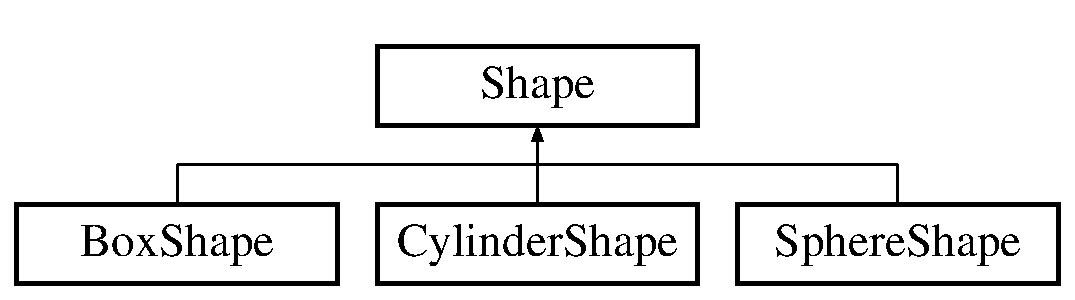
\includegraphics[height=2.000000cm]{class_shape}
\end{center}
\end{figure}
\subsection*{Public Member Functions}
\begin{DoxyCompactItemize}
\item 
virtual \mbox{\hyperlink{class_shape_ac8ad2fd02e1e94beeb98e65ab795cd56}{$\sim$\+Shape}} ()=default
\item 
bt\+Collision\+Shape $\ast$ \mbox{\hyperlink{class_shape_a0c6d149b79d77a23e32d915aa4b4aa30}{get}} ()
\end{DoxyCompactItemize}
\subsection*{Protected Member Functions}
\begin{DoxyCompactItemize}
\item 
\mbox{\hyperlink{class_shape_a70a5dc66f409ae0ddafb35927b091fec}{Shape}} (shared\+\_\+ptr$<$ bt\+Collision\+Shape $>$ \+\_\+shape)
\end{DoxyCompactItemize}
\subsection*{Protected Attributes}
\begin{DoxyCompactItemize}
\item 
shared\+\_\+ptr$<$ bt\+Collision\+Shape $>$ \mbox{\hyperlink{class_shape_a2dfbbc42dde579257637148489c1fb9b}{shape}}
\end{DoxyCompactItemize}


\subsection{Constructor \& Destructor Documentation}
\mbox{\Hypertarget{class_shape_ac8ad2fd02e1e94beeb98e65ab795cd56}\label{class_shape_ac8ad2fd02e1e94beeb98e65ab795cd56}} 
\index{Shape@{Shape}!````~Shape@{$\sim$\+Shape}}
\index{````~Shape@{$\sim$\+Shape}!Shape@{Shape}}
\subsubsection{\texorpdfstring{$\sim$\+Shape()}{~Shape()}}
{\footnotesize\ttfamily virtual Shape\+::$\sim$\+Shape (\begin{DoxyParamCaption}{ }\end{DoxyParamCaption})\hspace{0.3cm}{\ttfamily [virtual]}, {\ttfamily [default]}}

\mbox{\Hypertarget{class_shape_a70a5dc66f409ae0ddafb35927b091fec}\label{class_shape_a70a5dc66f409ae0ddafb35927b091fec}} 
\index{Shape@{Shape}!Shape@{Shape}}
\index{Shape@{Shape}!Shape@{Shape}}
\subsubsection{\texorpdfstring{Shape()}{Shape()}}
{\footnotesize\ttfamily Shape\+::\+Shape (\begin{DoxyParamCaption}\item[{shared\+\_\+ptr$<$ bt\+Collision\+Shape $>$}]{\+\_\+shape }\end{DoxyParamCaption})\hspace{0.3cm}{\ttfamily [inline]}, {\ttfamily [protected]}}



\subsection{Member Function Documentation}
\mbox{\Hypertarget{class_shape_a0c6d149b79d77a23e32d915aa4b4aa30}\label{class_shape_a0c6d149b79d77a23e32d915aa4b4aa30}} 
\index{Shape@{Shape}!get@{get}}
\index{get@{get}!Shape@{Shape}}
\subsubsection{\texorpdfstring{get()}{get()}}
{\footnotesize\ttfamily bt\+Collision\+Shape$\ast$ Shape\+::get (\begin{DoxyParamCaption}{ }\end{DoxyParamCaption})\hspace{0.3cm}{\ttfamily [inline]}}



\subsection{Member Data Documentation}
\mbox{\Hypertarget{class_shape_a2dfbbc42dde579257637148489c1fb9b}\label{class_shape_a2dfbbc42dde579257637148489c1fb9b}} 
\index{Shape@{Shape}!shape@{shape}}
\index{shape@{shape}!Shape@{Shape}}
\subsubsection{\texorpdfstring{shape}{shape}}
{\footnotesize\ttfamily shared\+\_\+ptr$<$ bt\+Collision\+Shape $>$ Shape\+::shape\hspace{0.3cm}{\ttfamily [protected]}}



The documentation for this class was generated from the following file\+:\begin{DoxyCompactItemize}
\item 
3d/1 rigid bodies/code/\+Headers/\mbox{\hyperlink{_shape_8hpp}{Shape.\+hpp}}\end{DoxyCompactItemize}

\hypertarget{class_sphere_shape}{}\section{Sphere\+Shape Class Reference}
\label{class_sphere_shape}\index{Sphere\+Shape@{Sphere\+Shape}}


{\ttfamily \#include $<$Sphere\+Shape.\+hpp$>$}

Inheritance diagram for Sphere\+Shape\+:\begin{figure}[H]
\begin{center}
\leavevmode
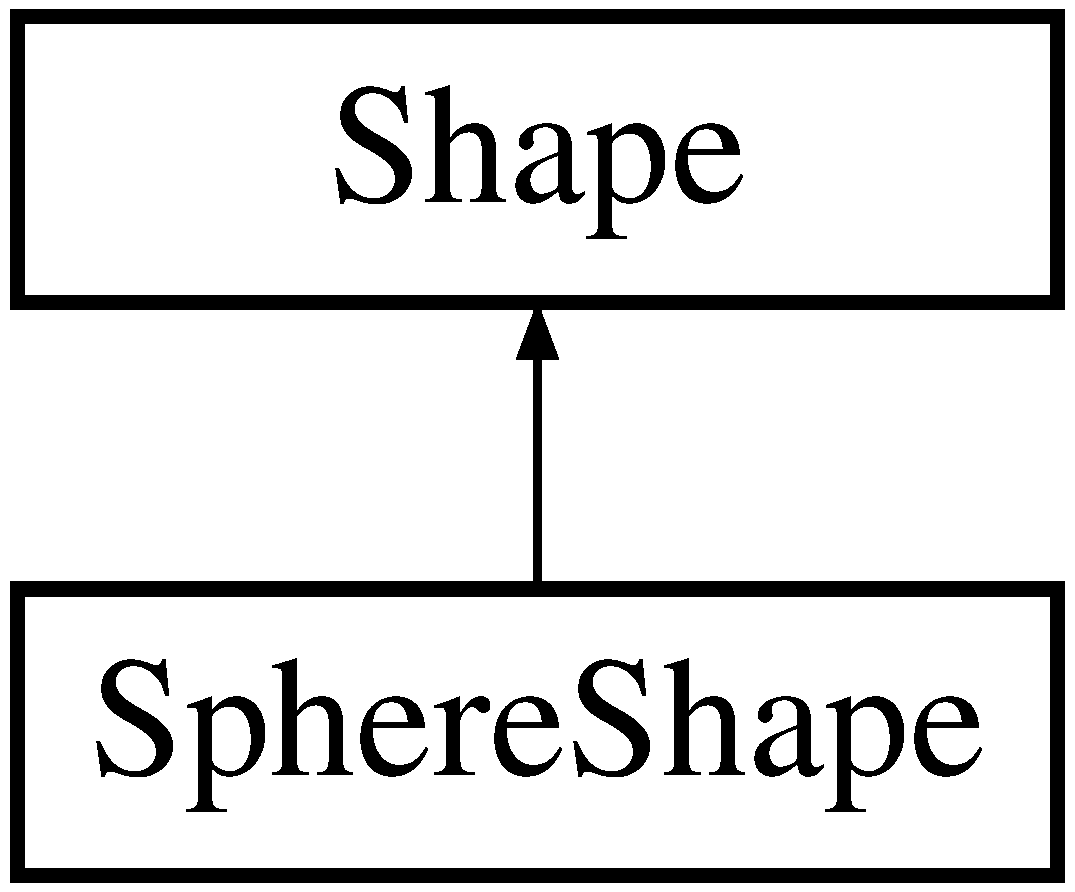
\includegraphics[height=2.000000cm]{class_sphere_shape}
\end{center}
\end{figure}
\subsection*{Public Member Functions}
\begin{DoxyCompactItemize}
\item 
\mbox{\hyperlink{class_sphere_shape_a4bba1b6e5fffae3e581aca4bb8d29d59}{Sphere\+Shape}} (float radius)
\end{DoxyCompactItemize}
\subsection*{Additional Inherited Members}


\subsection{Constructor \& Destructor Documentation}
\mbox{\Hypertarget{class_sphere_shape_a4bba1b6e5fffae3e581aca4bb8d29d59}\label{class_sphere_shape_a4bba1b6e5fffae3e581aca4bb8d29d59}} 
\index{Sphere\+Shape@{Sphere\+Shape}!Sphere\+Shape@{Sphere\+Shape}}
\index{Sphere\+Shape@{Sphere\+Shape}!Sphere\+Shape@{Sphere\+Shape}}
\subsubsection{\texorpdfstring{Sphere\+Shape()}{SphereShape()}}
{\footnotesize\ttfamily Sphere\+Shape\+::\+Sphere\+Shape (\begin{DoxyParamCaption}\item[{float}]{radius }\end{DoxyParamCaption})\hspace{0.3cm}{\ttfamily [inline]}}



The documentation for this class was generated from the following file\+:\begin{DoxyCompactItemize}
\item 
3d/1 rigid bodies/code/\+Headers/\mbox{\hyperlink{_sphere_shape_8hpp}{Sphere\+Shape.\+hpp}}\end{DoxyCompactItemize}

\hypertarget{class_tank}{}\section{Tank Class Reference}
\label{class_tank}\index{Tank@{Tank}}


{\ttfamily \#include $<$Tank.\+hpp$>$}

Inheritance diagram for Tank\+:\begin{figure}[H]
\begin{center}
\leavevmode
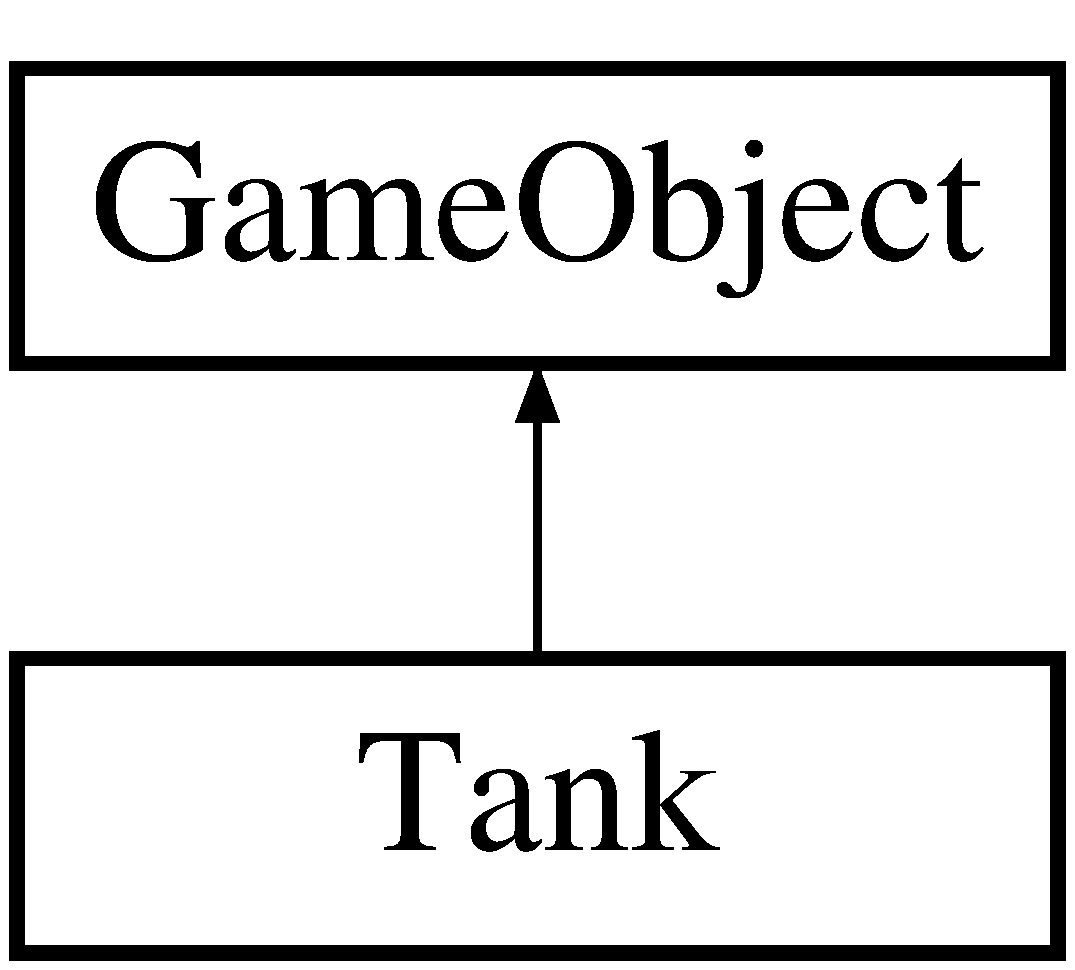
\includegraphics[height=2.000000cm]{class_tank}
\end{center}
\end{figure}
\subsection*{Public Member Functions}
\begin{DoxyCompactItemize}
\item 
\mbox{\hyperlink{class_tank_a7eec1b8b0587dff258a1ea2b66b85be1}{Tank}} (\mbox{\hyperlink{class_scene}{Scene}} \&\mbox{\hyperlink{class_game_object_aeea61de934e13603696b4ed00e9fe42e}{scene}})
\item 
void \mbox{\hyperlink{class_tank_a9628f999ddc963311cebf069da363d5c}{render}} () override
\end{DoxyCompactItemize}
\subsection*{Additional Inherited Members}


\subsection{Constructor \& Destructor Documentation}
\mbox{\Hypertarget{class_tank_a7eec1b8b0587dff258a1ea2b66b85be1}\label{class_tank_a7eec1b8b0587dff258a1ea2b66b85be1}} 
\index{Tank@{Tank}!Tank@{Tank}}
\index{Tank@{Tank}!Tank@{Tank}}
\subsubsection{\texorpdfstring{Tank()}{Tank()}}
{\footnotesize\ttfamily Tank\+::\+Tank (\begin{DoxyParamCaption}\item[{\mbox{\hyperlink{class_scene}{Scene}} \&}]{scene }\end{DoxyParamCaption})}



\subsection{Member Function Documentation}
\mbox{\Hypertarget{class_tank_a9628f999ddc963311cebf069da363d5c}\label{class_tank_a9628f999ddc963311cebf069da363d5c}} 
\index{Tank@{Tank}!render@{render}}
\index{render@{render}!Tank@{Tank}}
\subsubsection{\texorpdfstring{render()}{render()}}
{\footnotesize\ttfamily void Tank\+::render (\begin{DoxyParamCaption}{ }\end{DoxyParamCaption})\hspace{0.3cm}{\ttfamily [override]}, {\ttfamily [virtual]}}



Implements \mbox{\hyperlink{class_game_object_adee58d508cfa907162d1192a25dc21b9}{Game\+Object}}.



The documentation for this class was generated from the following file\+:\begin{DoxyCompactItemize}
\item 
3d/1 rigid bodies/code/\+Headers/\mbox{\hyperlink{_tank_8hpp}{Tank.\+hpp}}\end{DoxyCompactItemize}

\hypertarget{class_targets}{}\section{Targets Class Reference}
\label{class_targets}\index{Targets@{Targets}}


{\ttfamily \#include $<$Targets.\+hpp$>$}

Inheritance diagram for Targets\+:\begin{figure}[H]
\begin{center}
\leavevmode
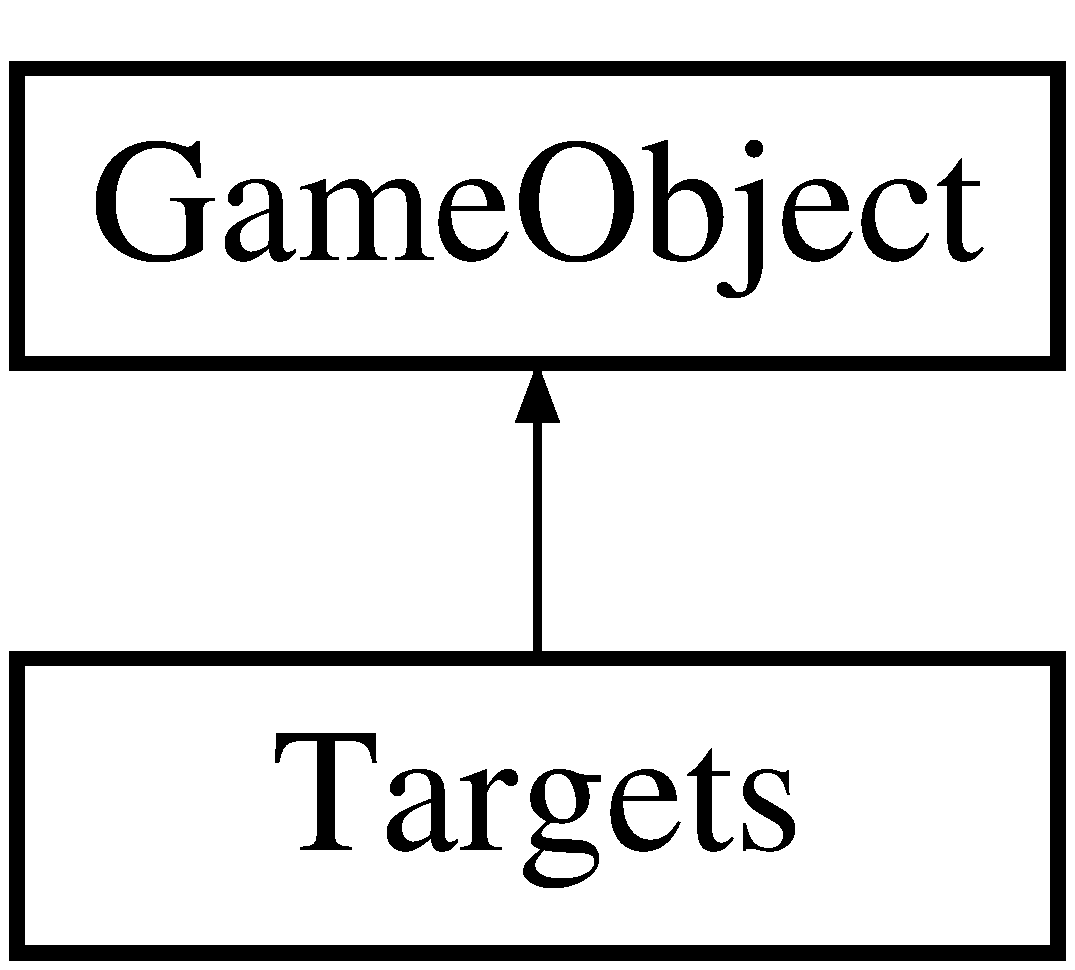
\includegraphics[height=2.000000cm]{class_targets}
\end{center}
\end{figure}
\subsection*{Public Member Functions}
\begin{DoxyCompactItemize}
\item 
\mbox{\hyperlink{class_targets_a4ab549593a5291fcd1e56adc97656acd}{Targets}} (\mbox{\hyperlink{class_scene}{Scene}} \&\mbox{\hyperlink{class_game_object_aeea61de934e13603696b4ed00e9fe42e}{scene}})
\item 
void \mbox{\hyperlink{class_targets_ae4f6dccb119a885728dc9e9c3e287c95}{render}} () override
\end{DoxyCompactItemize}
\subsection*{Additional Inherited Members}


\subsection{Constructor \& Destructor Documentation}
\mbox{\Hypertarget{class_targets_a4ab549593a5291fcd1e56adc97656acd}\label{class_targets_a4ab549593a5291fcd1e56adc97656acd}} 
\index{Targets@{Targets}!Targets@{Targets}}
\index{Targets@{Targets}!Targets@{Targets}}
\subsubsection{\texorpdfstring{Targets()}{Targets()}}
{\footnotesize\ttfamily Targets\+::\+Targets (\begin{DoxyParamCaption}\item[{\mbox{\hyperlink{class_scene}{Scene}} \&}]{scene }\end{DoxyParamCaption})}



\subsection{Member Function Documentation}
\mbox{\Hypertarget{class_targets_ae4f6dccb119a885728dc9e9c3e287c95}\label{class_targets_ae4f6dccb119a885728dc9e9c3e287c95}} 
\index{Targets@{Targets}!render@{render}}
\index{render@{render}!Targets@{Targets}}
\subsubsection{\texorpdfstring{render()}{render()}}
{\footnotesize\ttfamily void Targets\+::render (\begin{DoxyParamCaption}{ }\end{DoxyParamCaption})\hspace{0.3cm}{\ttfamily [override]}, {\ttfamily [virtual]}}



Implements \mbox{\hyperlink{class_game_object_adee58d508cfa907162d1192a25dc21b9}{Game\+Object}}.



The documentation for this class was generated from the following file\+:\begin{DoxyCompactItemize}
\item 
3d/1 rigid bodies/code/\+Headers/\mbox{\hyperlink{_targets_8hpp}{Targets.\+hpp}}\end{DoxyCompactItemize}

\hypertarget{class_wall}{}\section{Wall Class Reference}
\label{class_wall}\index{Wall@{Wall}}


{\ttfamily \#include $<$Wall.\+hpp$>$}

Inheritance diagram for Wall\+:\begin{figure}[H]
\begin{center}
\leavevmode
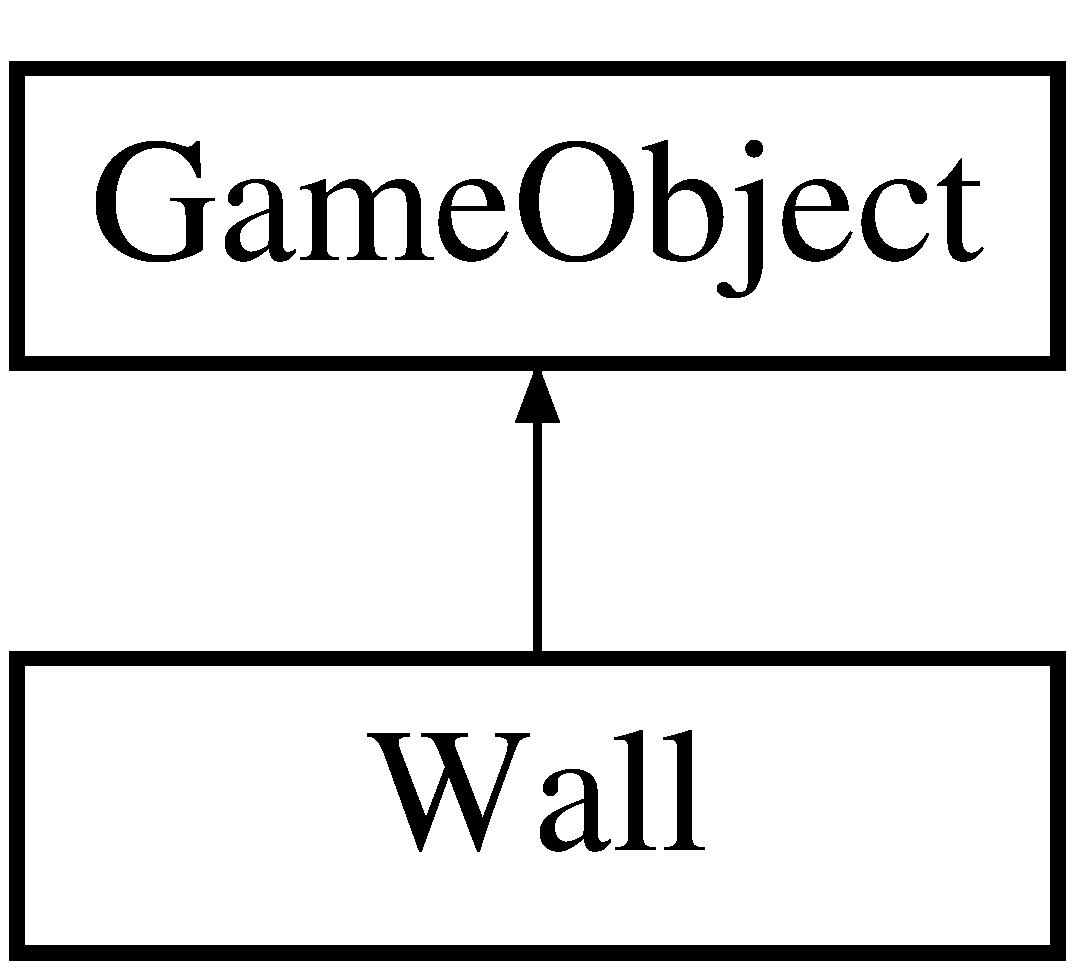
\includegraphics[height=2.000000cm]{class_wall}
\end{center}
\end{figure}
\subsection*{Public Member Functions}
\begin{DoxyCompactItemize}
\item 
\mbox{\hyperlink{class_wall_acff230e44e6b7210839291519052bd63}{Wall}} (\mbox{\hyperlink{class_scene}{Scene}} \&\mbox{\hyperlink{class_game_object_aeea61de934e13603696b4ed00e9fe42e}{scene}})
\item 
void \mbox{\hyperlink{class_wall_ad2b19eb994789ac7588b61a7ad0d928f}{render}} () override
\end{DoxyCompactItemize}
\subsection*{Additional Inherited Members}


\subsection{Constructor \& Destructor Documentation}
\mbox{\Hypertarget{class_wall_acff230e44e6b7210839291519052bd63}\label{class_wall_acff230e44e6b7210839291519052bd63}} 
\index{Wall@{Wall}!Wall@{Wall}}
\index{Wall@{Wall}!Wall@{Wall}}
\subsubsection{\texorpdfstring{Wall()}{Wall()}}
{\footnotesize\ttfamily Wall\+::\+Wall (\begin{DoxyParamCaption}\item[{\mbox{\hyperlink{class_scene}{Scene}} \&}]{scene }\end{DoxyParamCaption})}



\subsection{Member Function Documentation}
\mbox{\Hypertarget{class_wall_ad2b19eb994789ac7588b61a7ad0d928f}\label{class_wall_ad2b19eb994789ac7588b61a7ad0d928f}} 
\index{Wall@{Wall}!render@{render}}
\index{render@{render}!Wall@{Wall}}
\subsubsection{\texorpdfstring{render()}{render()}}
{\footnotesize\ttfamily void Wall\+::render (\begin{DoxyParamCaption}{ }\end{DoxyParamCaption})\hspace{0.3cm}{\ttfamily [override]}, {\ttfamily [virtual]}}



Implements \mbox{\hyperlink{class_game_object_adee58d508cfa907162d1192a25dc21b9}{Game\+Object}}.



The documentation for this class was generated from the following file\+:\begin{DoxyCompactItemize}
\item 
3d/1 rigid bodies/code/\+Headers/\mbox{\hyperlink{_wall_8hpp}{Wall.\+hpp}}\end{DoxyCompactItemize}

\chapter{File Documentation}
\hypertarget{_box_shape_8h}{}\section{3d/1 rigid bodies/code/\+Headers/\+Box\+Shape.h File Reference}
\label{_box_shape_8h}\index{3d/1 rigid bodies/code/\+Headers/\+Box\+Shape.\+h@{3d/1 rigid bodies/code/\+Headers/\+Box\+Shape.\+h}}

\hypertarget{_box_shape_8hpp}{}\section{3d/1 rigid bodies/code/\+Headers/\+Box\+Shape.hpp File Reference}
\label{_box_shape_8hpp}\index{3d/1 rigid bodies/code/\+Headers/\+Box\+Shape.\+hpp@{3d/1 rigid bodies/code/\+Headers/\+Box\+Shape.\+hpp}}
{\ttfamily \#include \char`\"{}Shape.\+hpp\char`\"{}}\newline
{\ttfamily \#include $<$bt\+Bullet\+Dynamics\+Common.\+h$>$}\newline
\subsection*{Classes}
\begin{DoxyCompactItemize}
\item 
class \mbox{\hyperlink{class_box_shape}{Box\+Shape}}
\end{DoxyCompactItemize}

\hypertarget{_bullet_8hpp}{}\section{3d/1 rigid bodies/code/\+Headers/\+Bullet.hpp File Reference}
\label{_bullet_8hpp}\index{3d/1 rigid bodies/code/\+Headers/\+Bullet.\+hpp@{3d/1 rigid bodies/code/\+Headers/\+Bullet.\+hpp}}
{\ttfamily \#include \char`\"{}Game\+Object.\+hpp\char`\"{}}\newline
{\ttfamily \#include \char`\"{}Box\+Shape.\+hpp\char`\"{}}\newline
{\ttfamily \#include \char`\"{}Sphere\+Shape.\+hpp\char`\"{}}\newline
{\ttfamily \#include \char`\"{}Rigidbody.\+hpp\char`\"{}}\newline
\subsection*{Classes}
\begin{DoxyCompactItemize}
\item 
class \mbox{\hyperlink{class_bullet}{Bullet}}
\end{DoxyCompactItemize}

\hypertarget{_cylinder_shape_8hpp}{}\section{3d/1 rigid bodies/code/\+Headers/\+Cylinder\+Shape.hpp File Reference}
\label{_cylinder_shape_8hpp}\index{3d/1 rigid bodies/code/\+Headers/\+Cylinder\+Shape.\+hpp@{3d/1 rigid bodies/code/\+Headers/\+Cylinder\+Shape.\+hpp}}
{\ttfamily \#include \char`\"{}Shape.\+hpp\char`\"{}}\newline
{\ttfamily \#include $<$bt\+Bullet\+Dynamics\+Common.\+h$>$}\newline
\subsection*{Classes}
\begin{DoxyCompactItemize}
\item 
class \mbox{\hyperlink{class_cylinder_shape}{Cylinder\+Shape}}
\end{DoxyCompactItemize}

\hypertarget{_demo_8hpp}{}\section{3d/1 rigid bodies/code/\+Headers/\+Demo.hpp File Reference}
\label{_demo_8hpp}\index{3d/1 rigid bodies/code/\+Headers/\+Demo.\+hpp@{3d/1 rigid bodies/code/\+Headers/\+Demo.\+hpp}}

\hypertarget{_floor_8hpp}{}\section{3d/1 rigid bodies/code/\+Headers/\+Floor.hpp File Reference}
\label{_floor_8hpp}\index{3d/1 rigid bodies/code/\+Headers/\+Floor.\+hpp@{3d/1 rigid bodies/code/\+Headers/\+Floor.\+hpp}}
{\ttfamily \#include \char`\"{}Game\+Object.\+hpp\char`\"{}}\newline
\subsection*{Classes}
\begin{DoxyCompactItemize}
\item 
class \mbox{\hyperlink{class_floor}{Floor}}
\end{DoxyCompactItemize}

\hypertarget{_game_object_8hpp}{}\section{3d/1 rigid bodies/code/\+Headers/\+Game\+Object.hpp File Reference}
\label{_game_object_8hpp}\index{3d/1 rigid bodies/code/\+Headers/\+Game\+Object.\+hpp@{3d/1 rigid bodies/code/\+Headers/\+Game\+Object.\+hpp}}
{\ttfamily \#include $<$memory$>$}\newline
{\ttfamily \#include \char`\"{}Shape.\+hpp\char`\"{}}\newline
{\ttfamily \#include \char`\"{}Rigidbody.\+hpp\char`\"{}}\newline
{\ttfamily \#include \char`\"{}Model\+\_\+\+Obj.\+hpp\char`\"{}}\newline
{\ttfamily \#include \char`\"{}Box\+Shape.\+hpp\char`\"{}}\newline
{\ttfamily \#include \char`\"{}Physics\+World.\+hpp\char`\"{}}\newline
{\ttfamily \#include $<$Render\+\_\+\+Node.\+hpp$>$}\newline
\subsection*{Classes}
\begin{DoxyCompactItemize}
\item 
class \mbox{\hyperlink{class_game_object}{Game\+Object}}
\item 
struct \mbox{\hyperlink{struct_game_object_1_1_parts}{Game\+Object\+::\+Parts}}
\end{DoxyCompactItemize}

\hypertarget{_key_8hpp}{}\section{3d/1 rigid bodies/code/\+Headers/\+Key.hpp File Reference}
\label{_key_8hpp}\index{3d/1 rigid bodies/code/\+Headers/\+Key.\+hpp@{3d/1 rigid bodies/code/\+Headers/\+Key.\+hpp}}
{\ttfamily \#include \char`\"{}Game\+Object.\+hpp\char`\"{}}\newline
{\ttfamily \#include \char`\"{}Box\+Shape.\+hpp\char`\"{}}\newline
{\ttfamily \#include \char`\"{}Sphere\+Shape.\+hpp\char`\"{}}\newline
{\ttfamily \#include \char`\"{}Rigidbody.\+hpp\char`\"{}}\newline
\subsection*{Classes}
\begin{DoxyCompactItemize}
\item 
class \mbox{\hyperlink{class_key}{Key}}
\end{DoxyCompactItemize}

\hypertarget{_physics_world_8hpp}{}\section{3d/1 rigid bodies/code/\+Headers/\+Physics\+World.hpp File Reference}
\label{_physics_world_8hpp}\index{3d/1 rigid bodies/code/\+Headers/\+Physics\+World.\+hpp@{3d/1 rigid bodies/code/\+Headers/\+Physics\+World.\+hpp}}
{\ttfamily \#include $<$bt\+Bullet\+Dynamics\+Common.\+h$>$}\newline
{\ttfamily \#include $<$memory$>$}\newline
{\ttfamily \#include $<$vector$>$}\newline
{\ttfamily \#include \char`\"{}Rigidbody.\+hpp\char`\"{}}\newline
\subsection*{Classes}
\begin{DoxyCompactItemize}
\item 
class \mbox{\hyperlink{class_physics_world}{Physics\+World}}
\end{DoxyCompactItemize}

\hypertarget{_platform_move_8hpp}{}\section{3d/1 rigid bodies/code/\+Headers/\+Platform\+Move.hpp File Reference}
\label{_platform_move_8hpp}\index{3d/1 rigid bodies/code/\+Headers/\+Platform\+Move.\+hpp@{3d/1 rigid bodies/code/\+Headers/\+Platform\+Move.\+hpp}}
{\ttfamily \#include \char`\"{}Game\+Object.\+hpp\char`\"{}}\newline
{\ttfamily \#include \char`\"{}Box\+Shape.\+hpp\char`\"{}}\newline
{\ttfamily \#include \char`\"{}Sphere\+Shape.\+hpp\char`\"{}}\newline
{\ttfamily \#include \char`\"{}Rigidbody.\+hpp\char`\"{}}\newline
\subsection*{Classes}
\begin{DoxyCompactItemize}
\item 
class \mbox{\hyperlink{class_platform_move}{Platform\+Move}}
\end{DoxyCompactItemize}

\hypertarget{_rigidbody_8hpp}{}\section{3d/1 rigid bodies/code/\+Headers/\+Rigidbody.hpp File Reference}
\label{_rigidbody_8hpp}\index{3d/1 rigid bodies/code/\+Headers/\+Rigidbody.\+hpp@{3d/1 rigid bodies/code/\+Headers/\+Rigidbody.\+hpp}}
{\ttfamily \#include \char`\"{}../../code/\+Headers/\+Shape.\+hpp\char`\"{}}\newline
{\ttfamily \#include $<$bt\+Bullet\+Dynamics\+Common.\+h$>$}\newline
{\ttfamily \#include $<$memory$>$}\newline
{\ttfamily \#include $<$vector$>$}\newline
{\ttfamily \#include $<$iostream$>$}\newline
\subsection*{Classes}
\begin{DoxyCompactItemize}
\item 
class \mbox{\hyperlink{class_rigidbody}{Rigidbody}}
\end{DoxyCompactItemize}

\hypertarget{_scene_8hpp}{}\section{3d/1 rigid bodies/code/\+Headers/\+Scene.hpp File Reference}
\label{_scene_8hpp}\index{3d/1 rigid bodies/code/\+Headers/\+Scene.\+hpp@{3d/1 rigid bodies/code/\+Headers/\+Scene.\+hpp}}
{\ttfamily \#include $<$map$>$}\newline
{\ttfamily \#include $<$memory$>$}\newline
{\ttfamily \#include $<$vector$>$}\newline
{\ttfamily \#include $<$iostream$>$}\newline
{\ttfamily \#include $<$Light.\+hpp$>$}\newline
{\ttfamily \#include $<$Model.\+hpp$>$}\newline
{\ttfamily \#include $<$Open\+G\+L.\+hpp$>$}\newline
{\ttfamily \#include $<$Model\+\_\+\+Obj.\+hpp$>$}\newline
{\ttfamily \#include $<$Render\+\_\+\+Node.\+hpp$>$}\newline
{\ttfamily \#include $<$S\+F\+M\+L/\+Window.\+hpp$>$}\newline
{\ttfamily \#include \char`\"{}Physics\+World.\+hpp\char`\"{}}\newline
{\ttfamily \#include \char`\"{}Game\+Object.\+hpp\char`\"{}}\newline
{\ttfamily \#include \char`\"{}Floor.\+hpp\char`\"{}}\newline
{\ttfamily \#include \char`\"{}Tank.\+hpp\char`\"{}}\newline
{\ttfamily \#include \char`\"{}Wall.\+hpp\char`\"{}}\newline
{\ttfamily \#include \char`\"{}Targets.\+hpp\char`\"{}}\newline
{\ttfamily \#include \char`\"{}Key.\+hpp\char`\"{}}\newline
{\ttfamily \#include \char`\"{}Platform\+Move.\+hpp\char`\"{}}\newline
\subsection*{Classes}
\begin{DoxyCompactItemize}
\item 
class \mbox{\hyperlink{class_scene}{Scene}}
\end{DoxyCompactItemize}

\hypertarget{_shape_8hpp}{}\section{3d/1 rigid bodies/code/\+Headers/\+Shape.hpp File Reference}
\label{_shape_8hpp}\index{3d/1 rigid bodies/code/\+Headers/\+Shape.\+hpp@{3d/1 rigid bodies/code/\+Headers/\+Shape.\+hpp}}
{\ttfamily \#include $<$bt\+Bullet\+Dynamics\+Common.\+h$>$}\newline
{\ttfamily \#include $<$memory$>$}\newline
\subsection*{Classes}
\begin{DoxyCompactItemize}
\item 
class \mbox{\hyperlink{class_shape}{Shape}}
\end{DoxyCompactItemize}

\hypertarget{_sphere_shape_8hpp}{}\section{3d/1 rigid bodies/code/\+Headers/\+Sphere\+Shape.hpp File Reference}
\label{_sphere_shape_8hpp}\index{3d/1 rigid bodies/code/\+Headers/\+Sphere\+Shape.\+hpp@{3d/1 rigid bodies/code/\+Headers/\+Sphere\+Shape.\+hpp}}
{\ttfamily \#include \char`\"{}Shape.\+hpp\char`\"{}}\newline
{\ttfamily \#include $<$bt\+Bullet\+Dynamics\+Common.\+h$>$}\newline
\subsection*{Classes}
\begin{DoxyCompactItemize}
\item 
class \mbox{\hyperlink{class_sphere_shape}{Sphere\+Shape}}
\end{DoxyCompactItemize}

\hypertarget{_tank_8hpp}{}\section{3d/1 rigid bodies/code/\+Headers/\+Tank.hpp File Reference}
\label{_tank_8hpp}\index{3d/1 rigid bodies/code/\+Headers/\+Tank.\+hpp@{3d/1 rigid bodies/code/\+Headers/\+Tank.\+hpp}}
{\ttfamily \#include \char`\"{}Game\+Object.\+hpp\char`\"{}}\newline
{\ttfamily \#include \char`\"{}Box\+Shape.\+hpp\char`\"{}}\newline
{\ttfamily \#include \char`\"{}Sphere\+Shape.\+hpp\char`\"{}}\newline
{\ttfamily \#include \char`\"{}Cylinder\+Shape.\+hpp\char`\"{}}\newline
{\ttfamily \#include \char`\"{}Rigidbody.\+hpp\char`\"{}}\newline
{\ttfamily \#include $<$S\+F\+M\+L\textbackslash{}\+Window.\+hpp$>$}\newline
{\ttfamily \#include $<$S\+F\+M\+L\textbackslash{}\+Graphics.\+hpp$>$}\newline
{\ttfamily \#include \char`\"{}Bullet.\+hpp\char`\"{}}\newline
\subsection*{Classes}
\begin{DoxyCompactItemize}
\item 
class \mbox{\hyperlink{class_tank}{Tank}}
\end{DoxyCompactItemize}

\hypertarget{_targets_8hpp}{}\section{3d/1 rigid bodies/code/\+Headers/\+Targets.hpp File Reference}
\label{_targets_8hpp}\index{3d/1 rigid bodies/code/\+Headers/\+Targets.\+hpp@{3d/1 rigid bodies/code/\+Headers/\+Targets.\+hpp}}
{\ttfamily \#include \char`\"{}Game\+Object.\+hpp\char`\"{}}\newline
{\ttfamily \#include \char`\"{}Box\+Shape.\+hpp\char`\"{}}\newline
{\ttfamily \#include \char`\"{}Sphere\+Shape.\+hpp\char`\"{}}\newline
{\ttfamily \#include \char`\"{}Rigidbody.\+hpp\char`\"{}}\newline
\subsection*{Classes}
\begin{DoxyCompactItemize}
\item 
class \mbox{\hyperlink{class_targets}{Targets}}
\end{DoxyCompactItemize}

\hypertarget{_wall_8hpp}{}\section{3d/1 rigid bodies/code/\+Headers/\+Wall.hpp File Reference}
\label{_wall_8hpp}\index{3d/1 rigid bodies/code/\+Headers/\+Wall.\+hpp@{3d/1 rigid bodies/code/\+Headers/\+Wall.\+hpp}}
{\ttfamily \#include \char`\"{}Game\+Object.\+hpp\char`\"{}}\newline
{\ttfamily \#include \char`\"{}Box\+Shape.\+hpp\char`\"{}}\newline
{\ttfamily \#include \char`\"{}Sphere\+Shape.\+hpp\char`\"{}}\newline
{\ttfamily \#include \char`\"{}Rigidbody.\+hpp\char`\"{}}\newline
\subsection*{Classes}
\begin{DoxyCompactItemize}
\item 
class \mbox{\hyperlink{class_wall}{Wall}}
\end{DoxyCompactItemize}

%--- End generated contents ---

% Index
\backmatter
\newpage
\phantomsection
\clearemptydoublepage
\addcontentsline{toc}{chapter}{Index}
\printindex

\end{document}
